 \documentclass[h]{article}
\usepackage[margin=0.5in]{geometry}
\usepackage{amsfonts} 
\usepackage{textcomp}
 
\usepackage{graphicx}
\usepackage{caption}
\usepackage{subcaption}
\usepackage{float} 
\usepackage{flafter}
\graphicspath{ {../results/vis/} }
\usepackage{adjustbox}


\newcommand{\cent}{\textcent \hspace{4pt}}
\title{CS 7641 Machine Learning \\ Assignment 4}
\date{Due Sunday April 22nd, 2018 11:59pm}
\author{Philip Bale \\ pbale3}

\begin{document}

\maketitle

\section*{Introduction}  
This assignment explores reinforcement learning.  It begins by choosing two 
Markov Decision Procceses (MDPs).  Both MDPs are solved using both value 
iteration and policy iteration, and the results are compared against each other. 
 Afterwards, Q-learning is applied to both problems and those results are then 
 compared to the original results.
 
\subsection*{Problems Chosen}
Gridworld path finding was chosen as the basis for the two Markov Decision Processes.  This 
was done for a few different reasons.  First, the ease in visual representation 
and understanding.  Second, path finding is a common problem in real-life that 
has applications from walking to work, to driving cross-country, etc.  Third, it 
is easy to scale the complexity of a grid as well as increase in the number of 
states.  Fourth, for a solveable grid, one or more optimal solutions must exist. 
 All-in-all, gridworld is great for demonstration reinforcement learning.
 \\ \\ % 30 walls
 The first gridworld problem is an ``easy'' configuration.  It has a 10x10 
 shape with 70 possible states.
% 47 walls
 \\ \\ 
 The second gridworld problem is a ``hard'' configuration.  It has a 20x20 
 shape with 353 possible states.  
 \\ \\
 Each gridworld has its start state is in the bottom left corner and 
 its end state is in the top right corner.  Various ``walls'' exist that force 
 the solution to optimize around.  Various states have negative rewards 
 assosciated with them and are color-coated in the state graphs below.
 
  \begin{figure}[H]
  \minipage{0.05\textwidth}
   \endminipage\hfill
  \minipage{0.45\textwidth}
      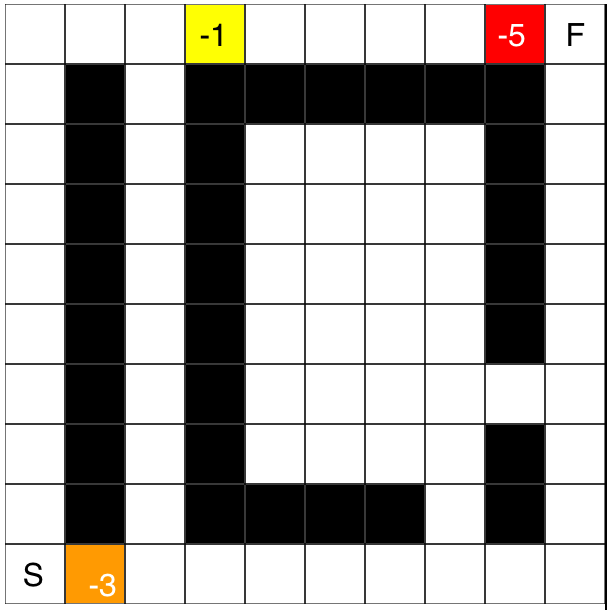
\includegraphics[width=1\textwidth,keepaspectratio]{easy-grid.png} 
      \caption*{10x10 Easy Gridworld w/ 70 States} 
   \endminipage\hfill
   \minipage{0.45\textwidth}
      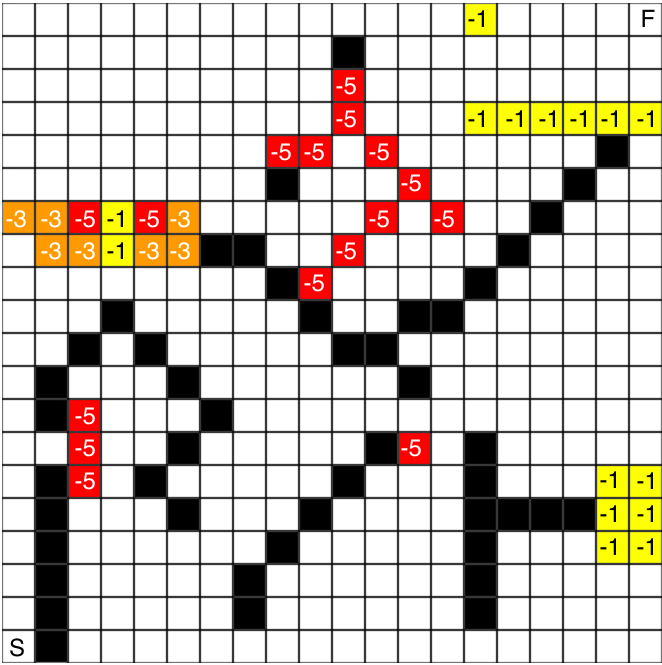
\includegraphics[width=1\textwidth,keepaspectratio]{hard-grid.png} 
      \caption*{20x20 Hard Gridworld w/ 353 States} 
   \endminipage\hfill
   \minipage{0.05\textwidth}
   \endminipage\hfill
\end{figure}


\section*{Value Iteration}
\subsection*{Introduction}
The first reinforcement learning algorithm used to optimally solve the MDPs is Value Iteration. 
 Value iteration works by using the Bellman equation while moving from 
 state to state in an attempt to reach convergence.  Since the utility is not 
 initially known, the algorithm begins with the reward at the final state and works 
 backwards calculating utility for nearest states.  This continues 
 until all states are evaluated.  After a number of iterations, the algorithm 
 will eventually converge on an optimal solution.
 
 
 \begin{figure}[H] 
\centering
\begin{tabular}{ | c | c  | c | c | c | c | c | c| c| c| c| c| c | } 
\hline
\textbf{Iterations} & \textbf{Time} & \textbf{Reward} & \textbf{Steps} & \textbf{Convergence}   \\
\hline
\textbf{EASY Gridworld} \\ \hline
1 & 0.0113 & -199.8800 & 197.4000 & 79.8000 \\ \hline
5 & 0.0545 & -18.6400 & 41.6200 & 20.6322 \\ \hline
10 & 0.1061 & 7.5400 & 24.5000 & 14.1408 \\ \hline
15 & 0.1575 & 34.8000 & 25.4400 & 6.9338 \\ \hline
25 & 0.2520 & 40.9400 & 28.4000 & 1.7116 \\ \hline
35 & 0.2954 & 45.4400 & 48.0800 & 0.0914 \\ \hline
45 & 0.3329 & 47.4400 & 44.5200 & 0.0010 \\ \hline
55 & 0.3735 & 46.0600 & 50.1800 & 2.89e-5 \\ \hline
60 & 0.3931 & 48.4400 & 48.1600 & 3.86e-6 \\ \hline
64 & 0.4090 & 50.0200 & 47.3800 & 8.78e-7 \\ \hline
\\
\textbf{HARD Gridworld} \\ \hline
1 & 0.0501 & -304.6200 & 300 & 83.8968 \\ \hline
5 & 0.1783 & -299 & 300 & 28.6170 \\ \hline
10 & 0.3105 & -299 & 300 & 14.2512 \\ \hline
20 & 0.5473 & -272.1300 & 282.6000 & 4.7330 \\ \hline
25 & 0.6585 & 7.1600 & 64.1800 & 2.7683 \\ \hline
35 & 0.8843 & 13.7700 & 63.4800 & 0.3277 \\ \hline
45 & 1.1318 & 9.1400 & 65.3000 & 0.0054 \\ \hline
55 & 1.3517 & 10.6000 & 63.7800 & 3.16e-5 \\ \hline
60 & 1.4623 & 13.2900 & 62.4400 & 1.72e-6 \\ \hline

\end{tabular}
\caption*{Gridworld Value Iteration Results} 
\end{figure}
 
 
   \begin{figure}[H]
  \minipage{0.245\textwidth}
      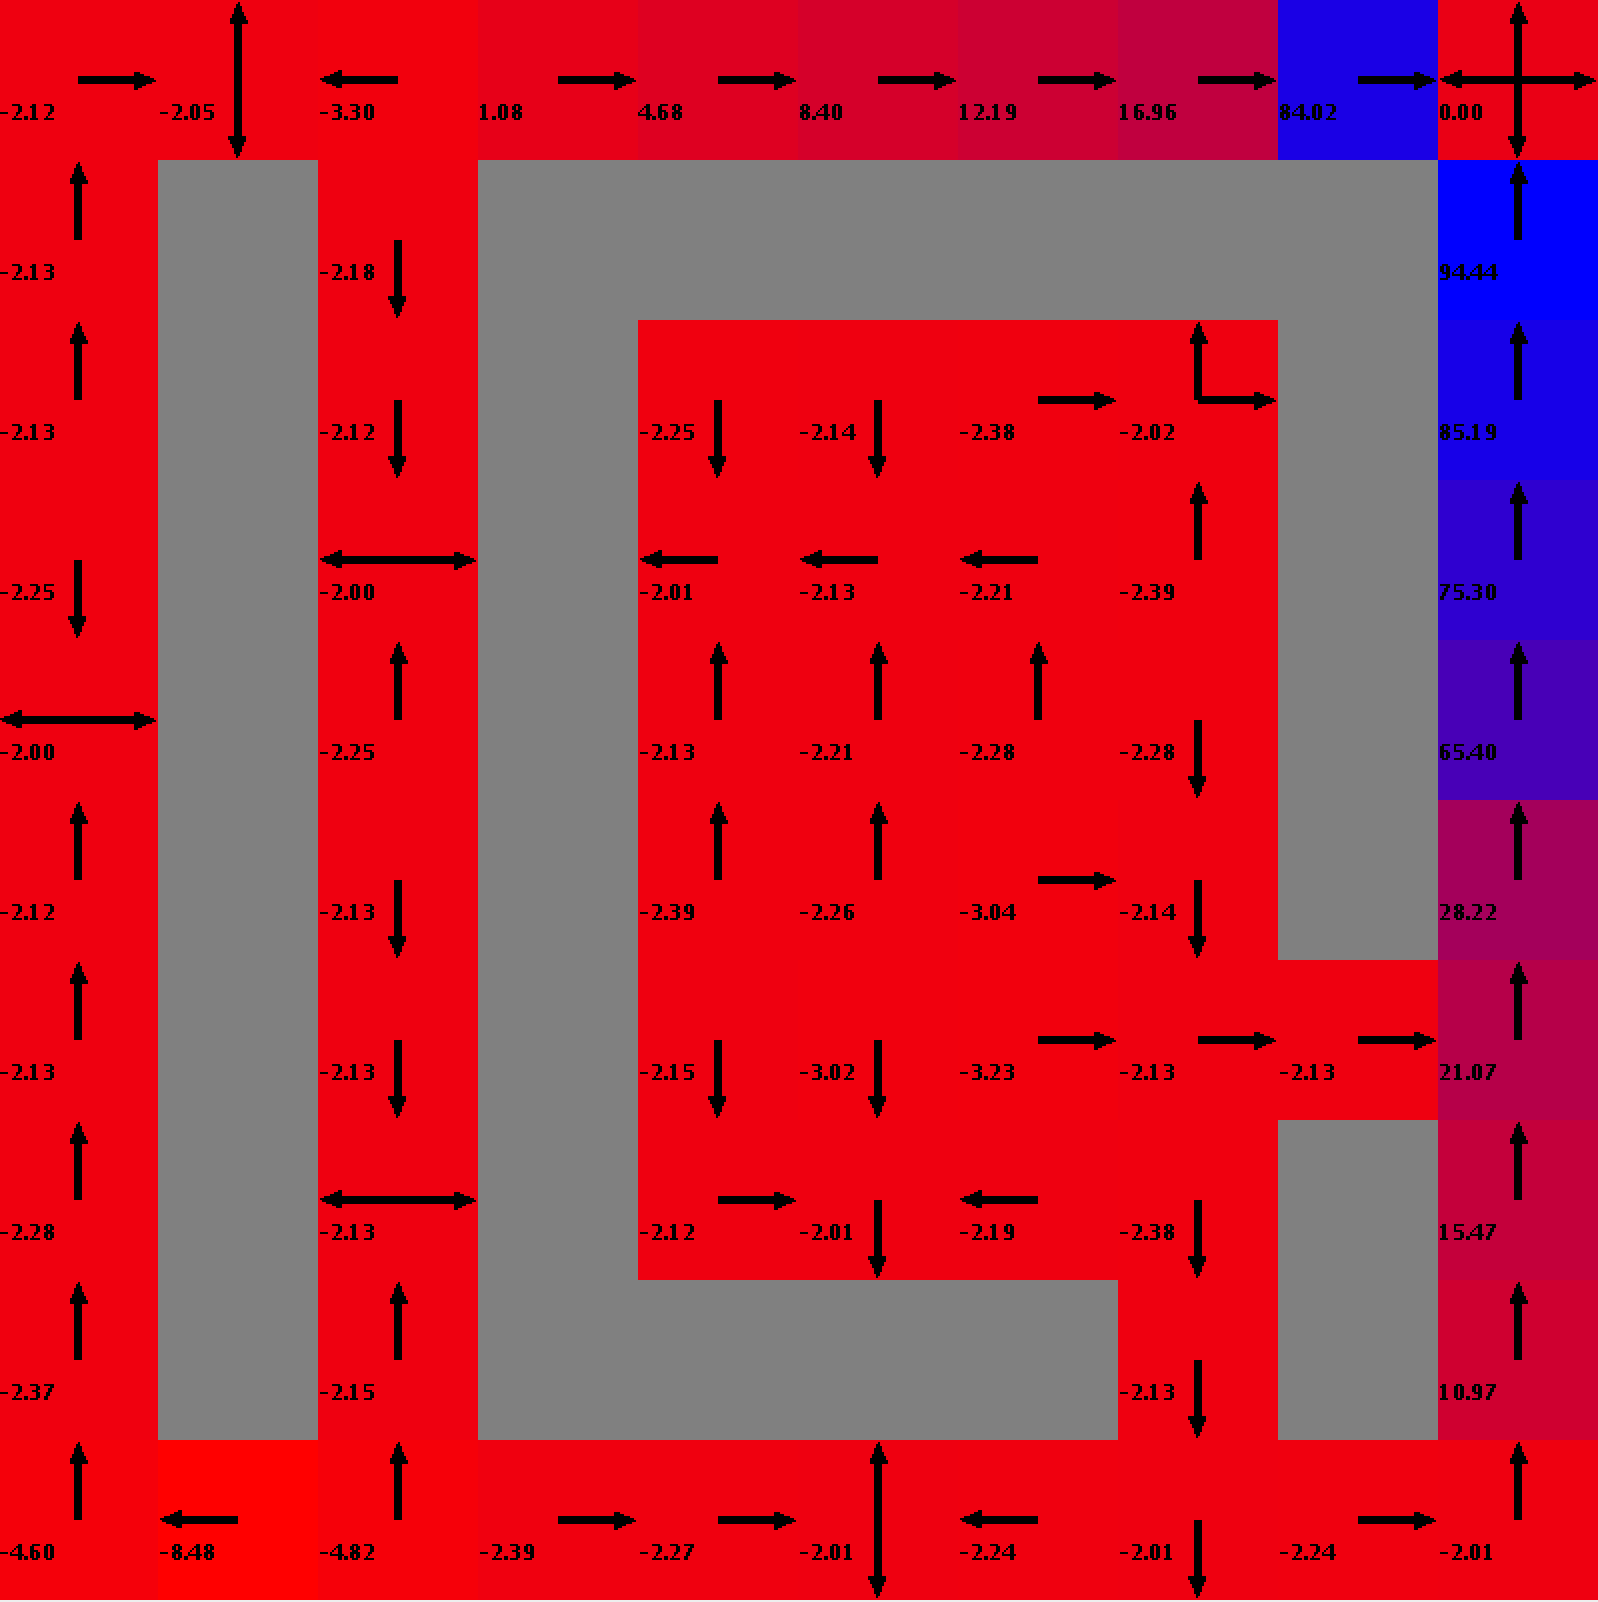
\includegraphics[width=1\textwidth,keepaspectratio]{easy-value-2.png} 
      \caption*{Easy GW Value Iteration \#2} 
   \endminipage\hfill
   \minipage{0.245\textwidth}
      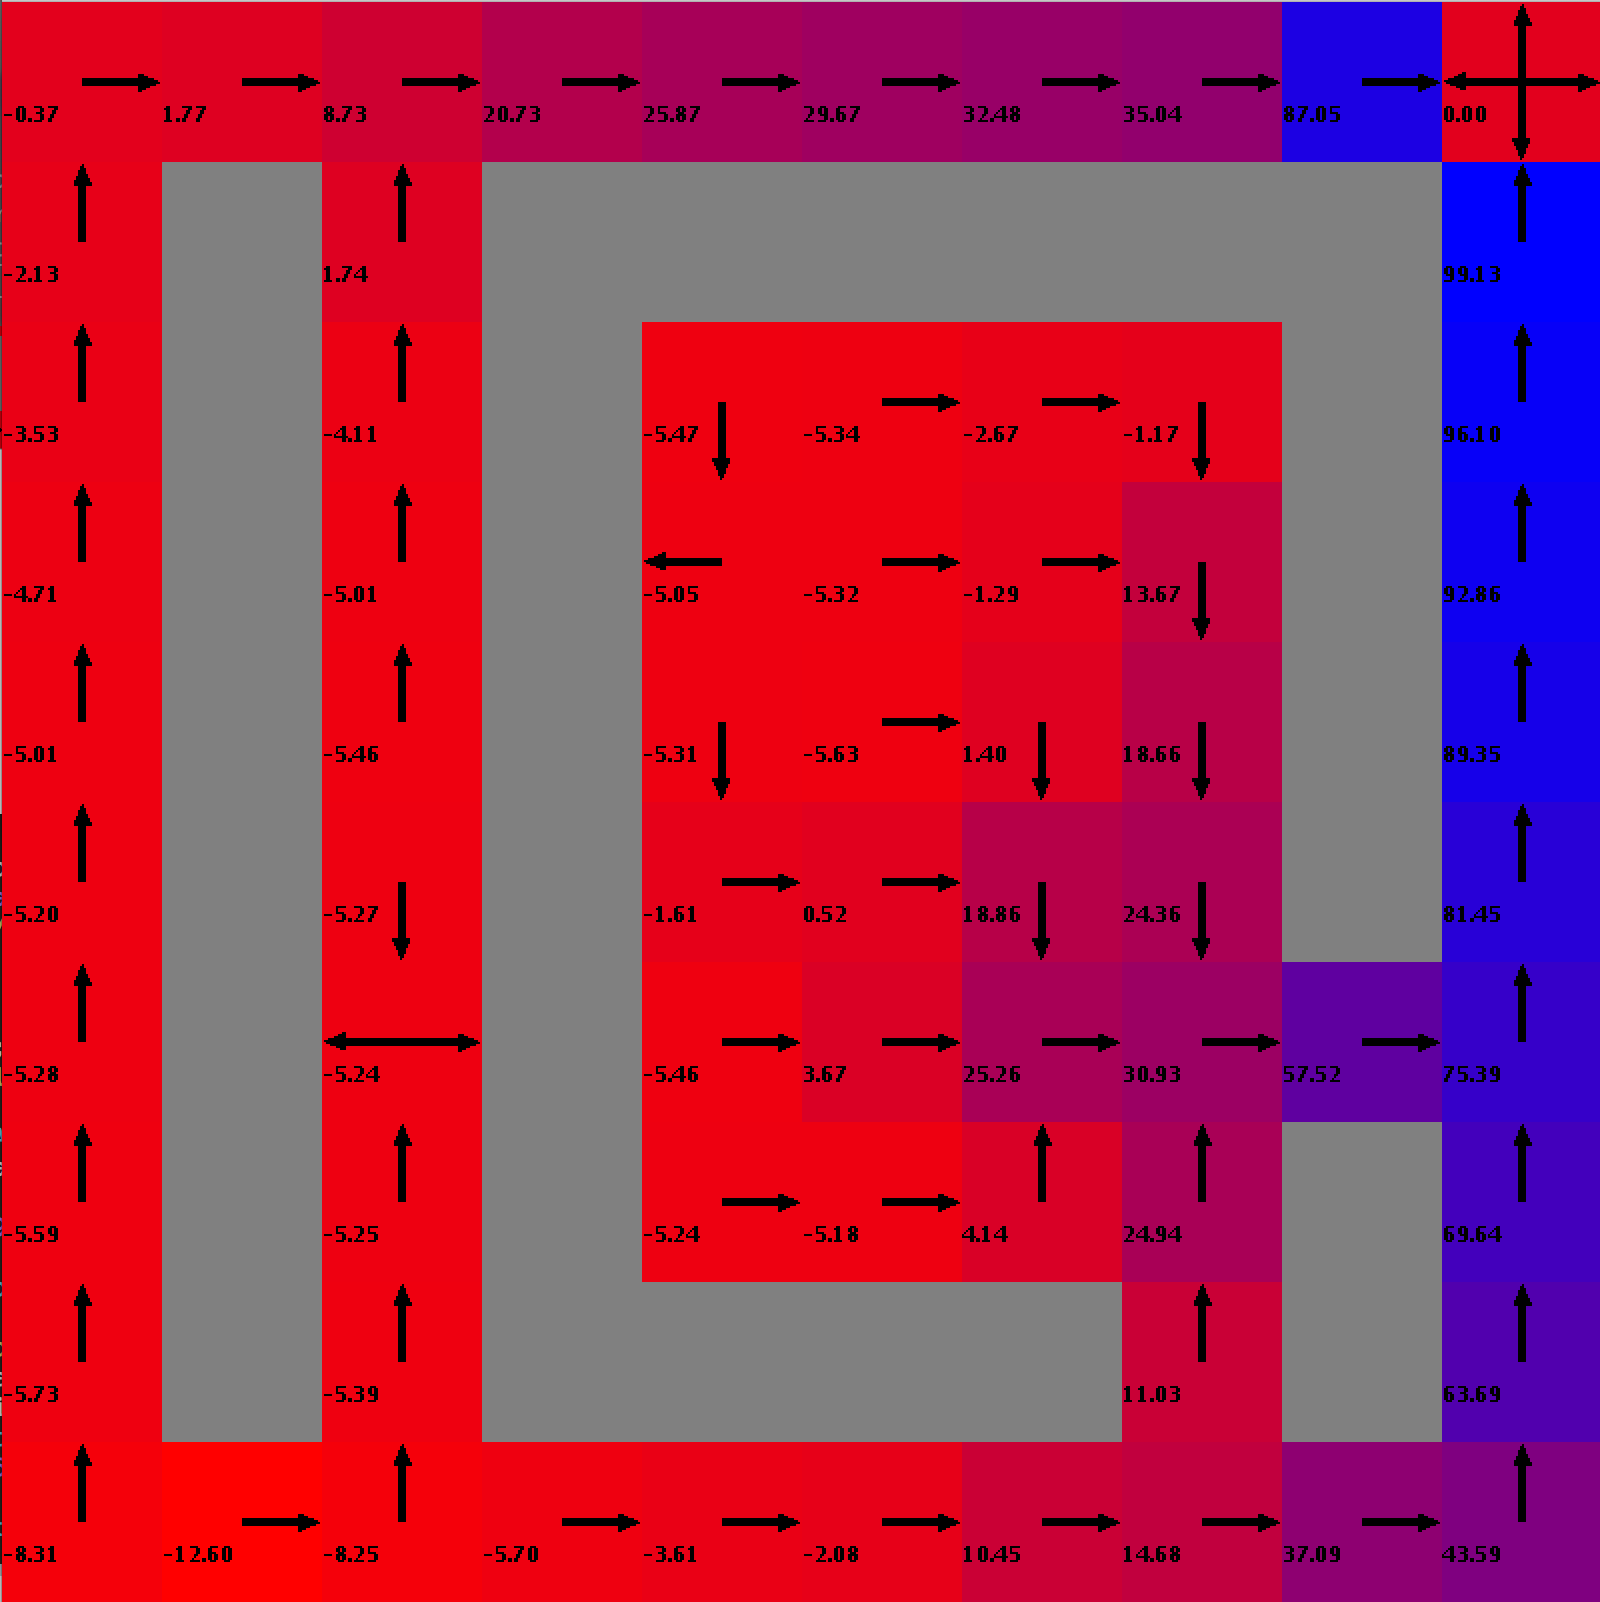
\includegraphics[width=1\textwidth,keepaspectratio]{easy-value-5.png} 
      \caption*{Easy GW Value Iteration \#5} 
   \endminipage\hfill
   \minipage{0.245\textwidth}
      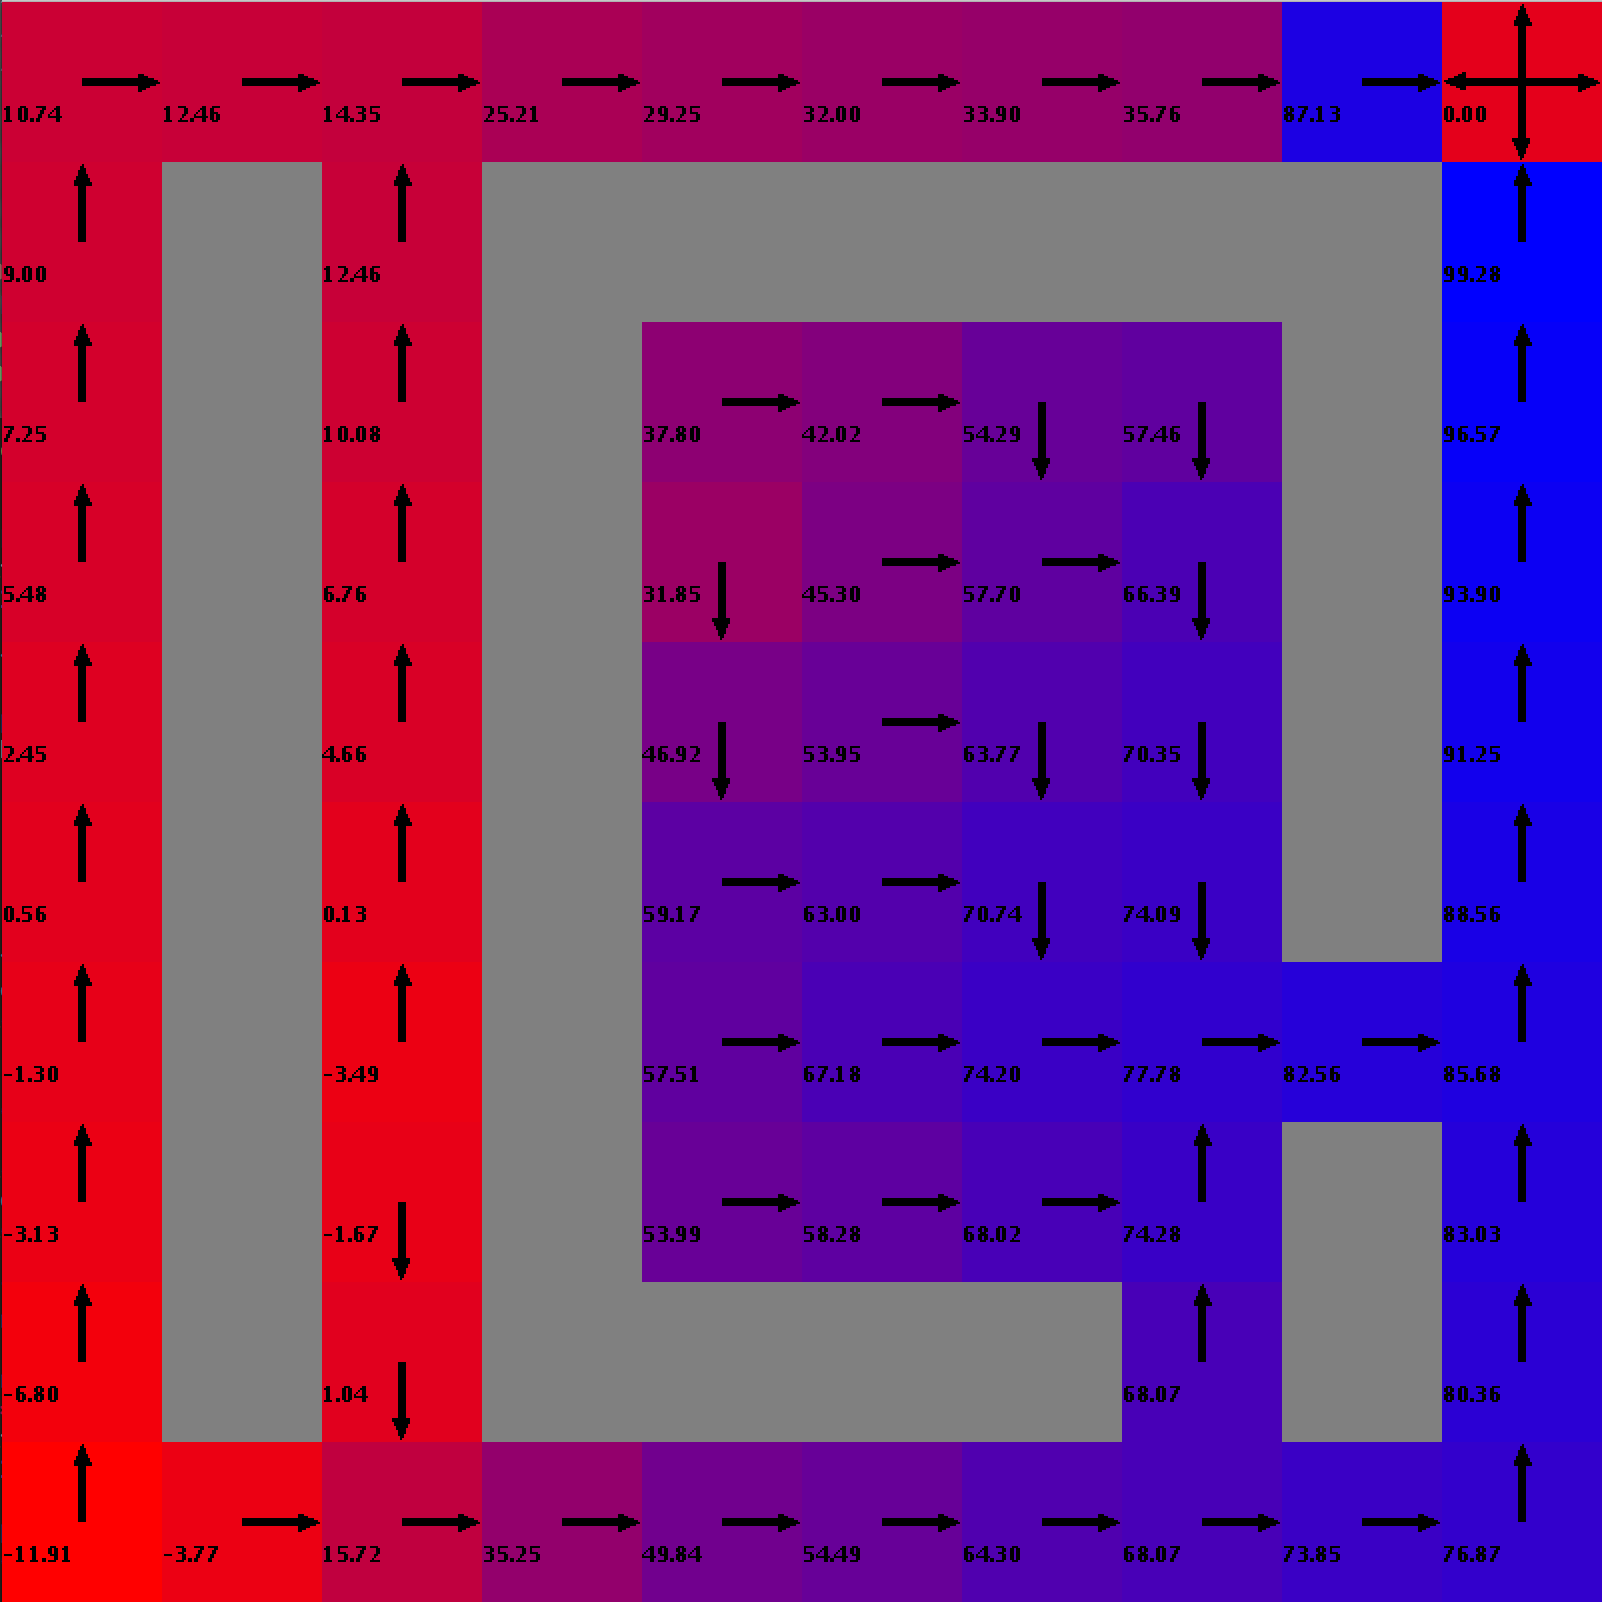
\includegraphics[width=1\textwidth,keepaspectratio]{easy-value-10.png} 
      \caption*{Easy GW Value Iteration \#10} 
   \endminipage\hfill
   \minipage{0.245\textwidth}
      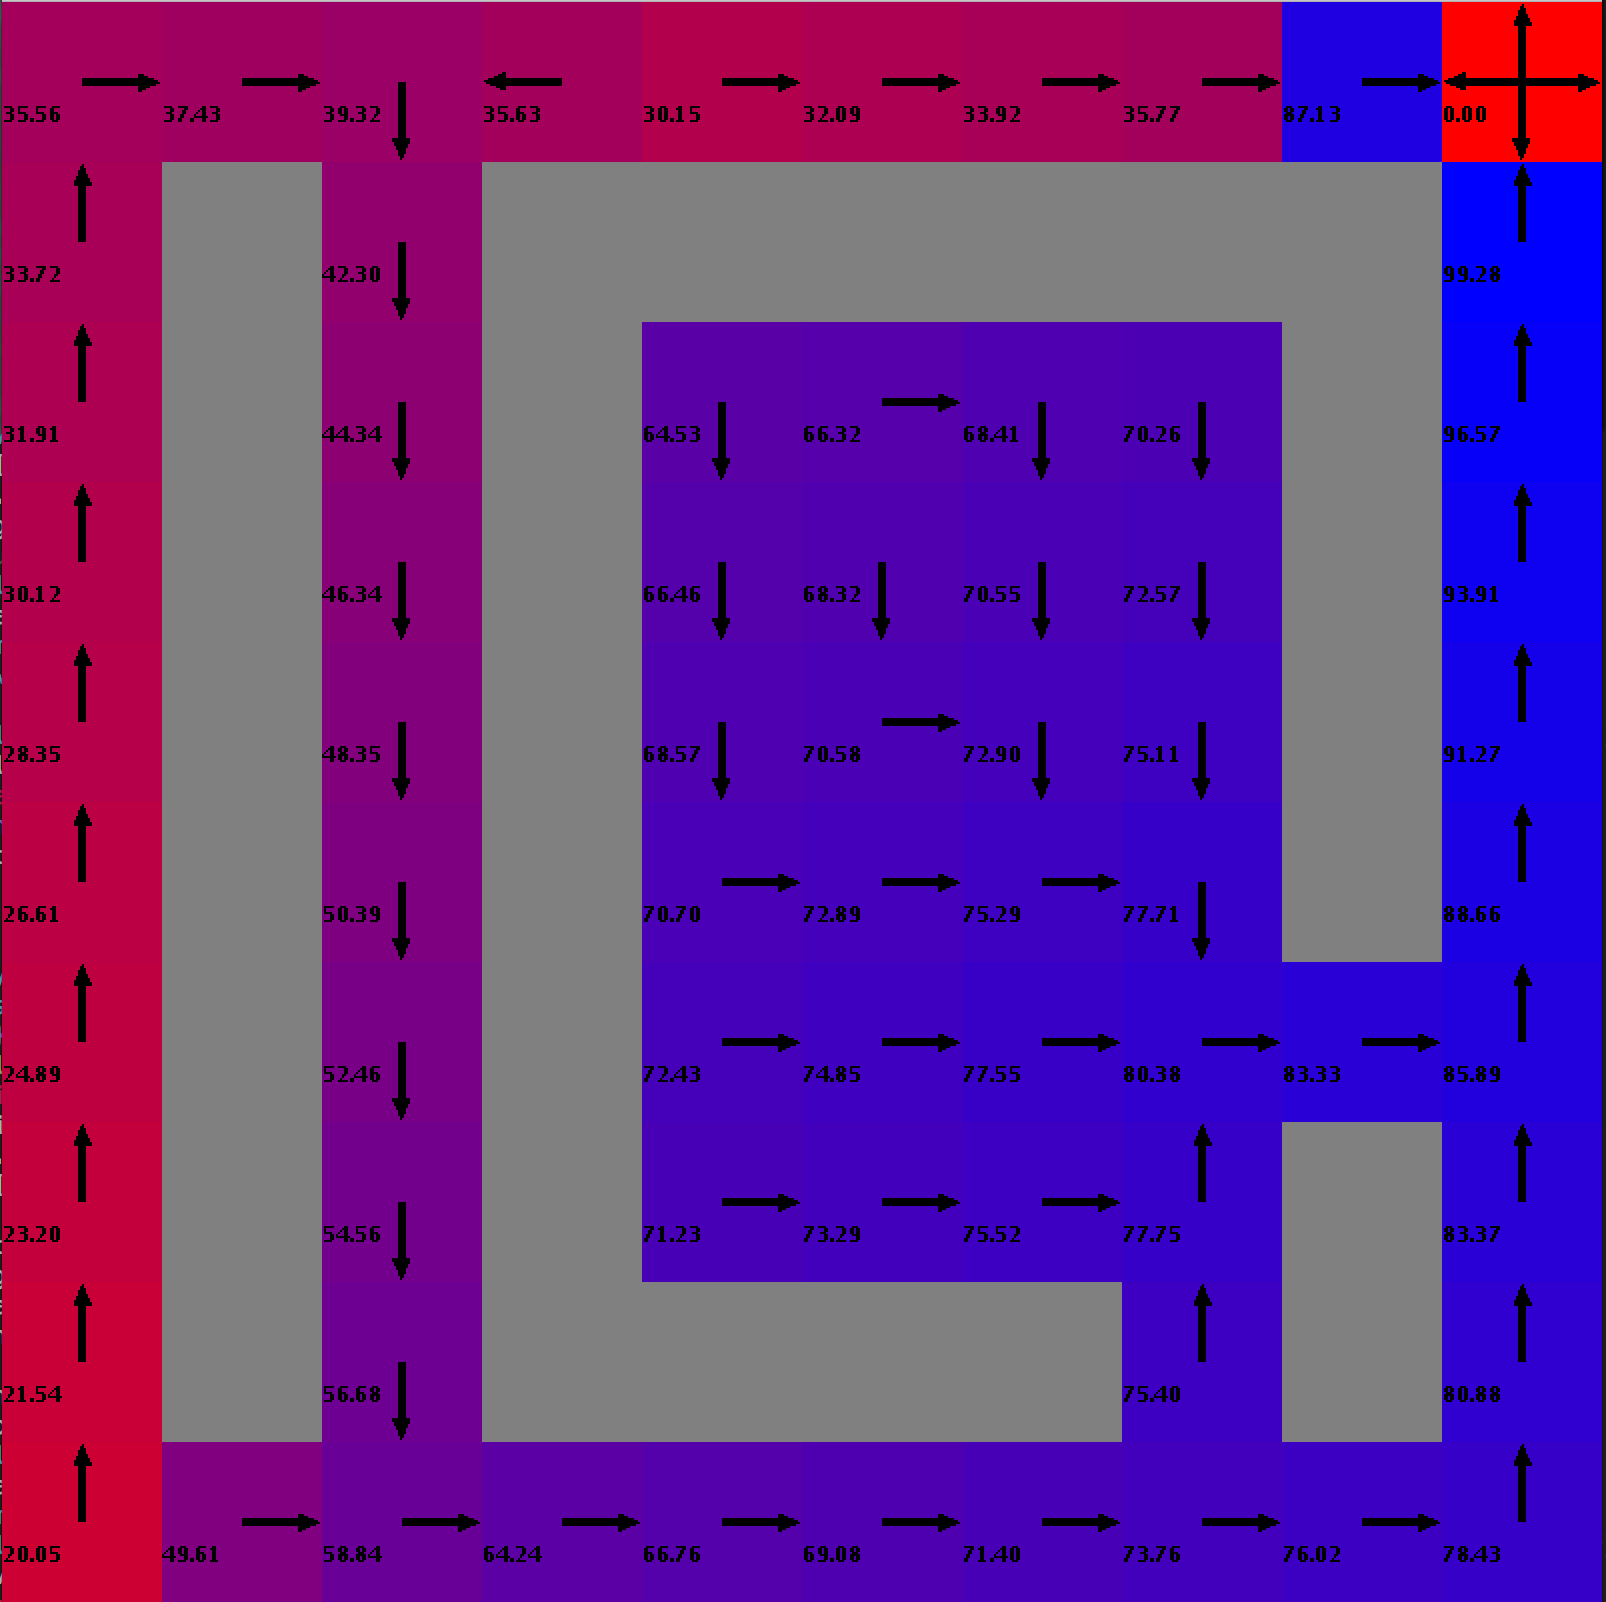
\includegraphics[width=1\textwidth,keepaspectratio]{easy-value-64.png} 
      \caption*{Easy GW Value Iteration \#64} 
   \endminipage\hfill
\end{figure}


   \begin{figure}[H]
  \minipage{0.245\textwidth}
      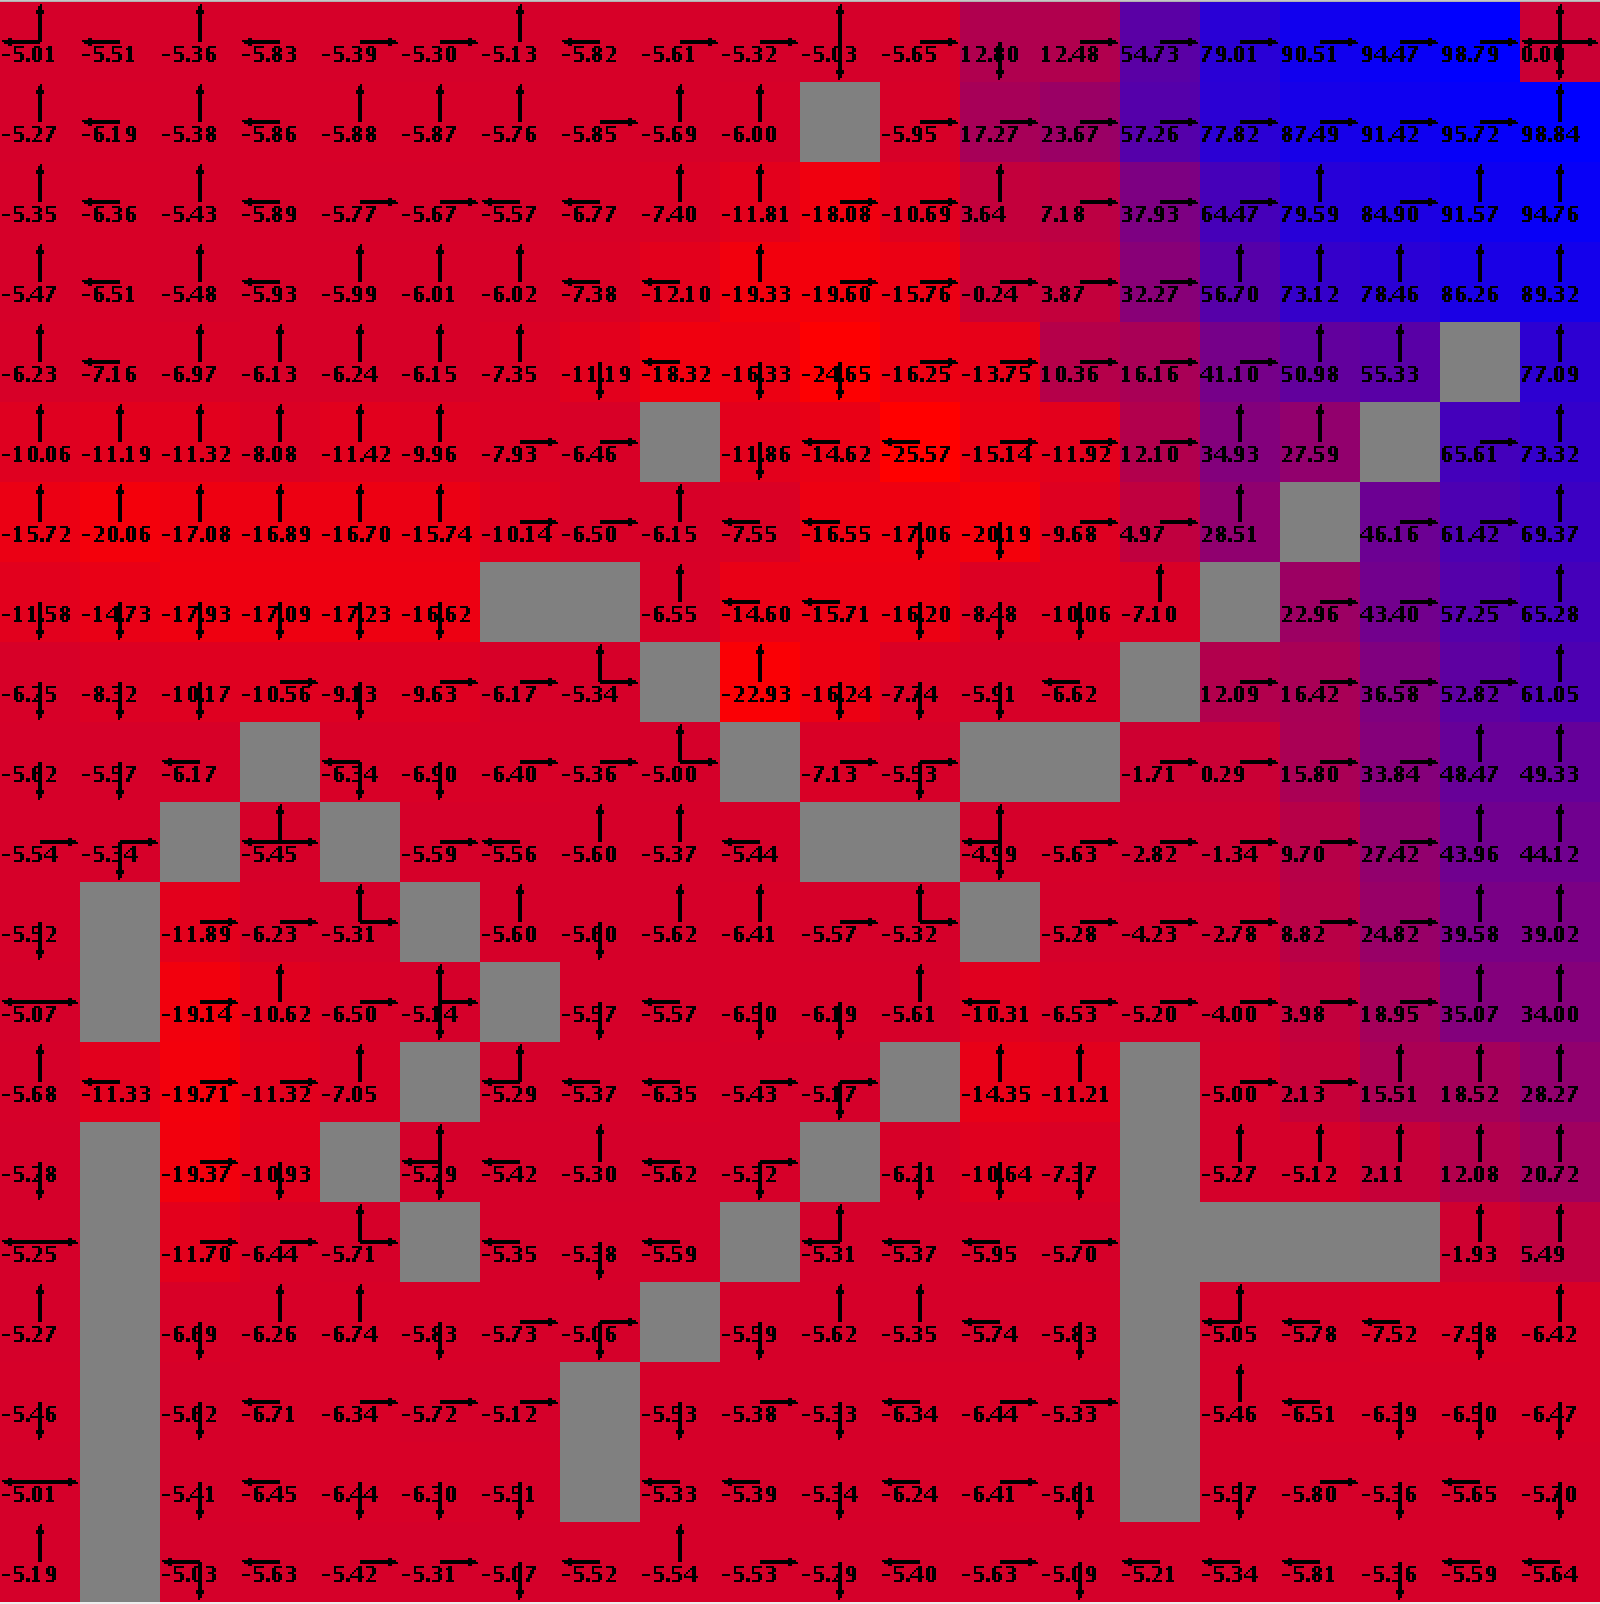
\includegraphics[width=1\textwidth,keepaspectratio]{hard-value-5.png} 
      \caption*{Hard GW Value Iteration \#5} 
   \endminipage\hfill
   \minipage{0.245\textwidth}
      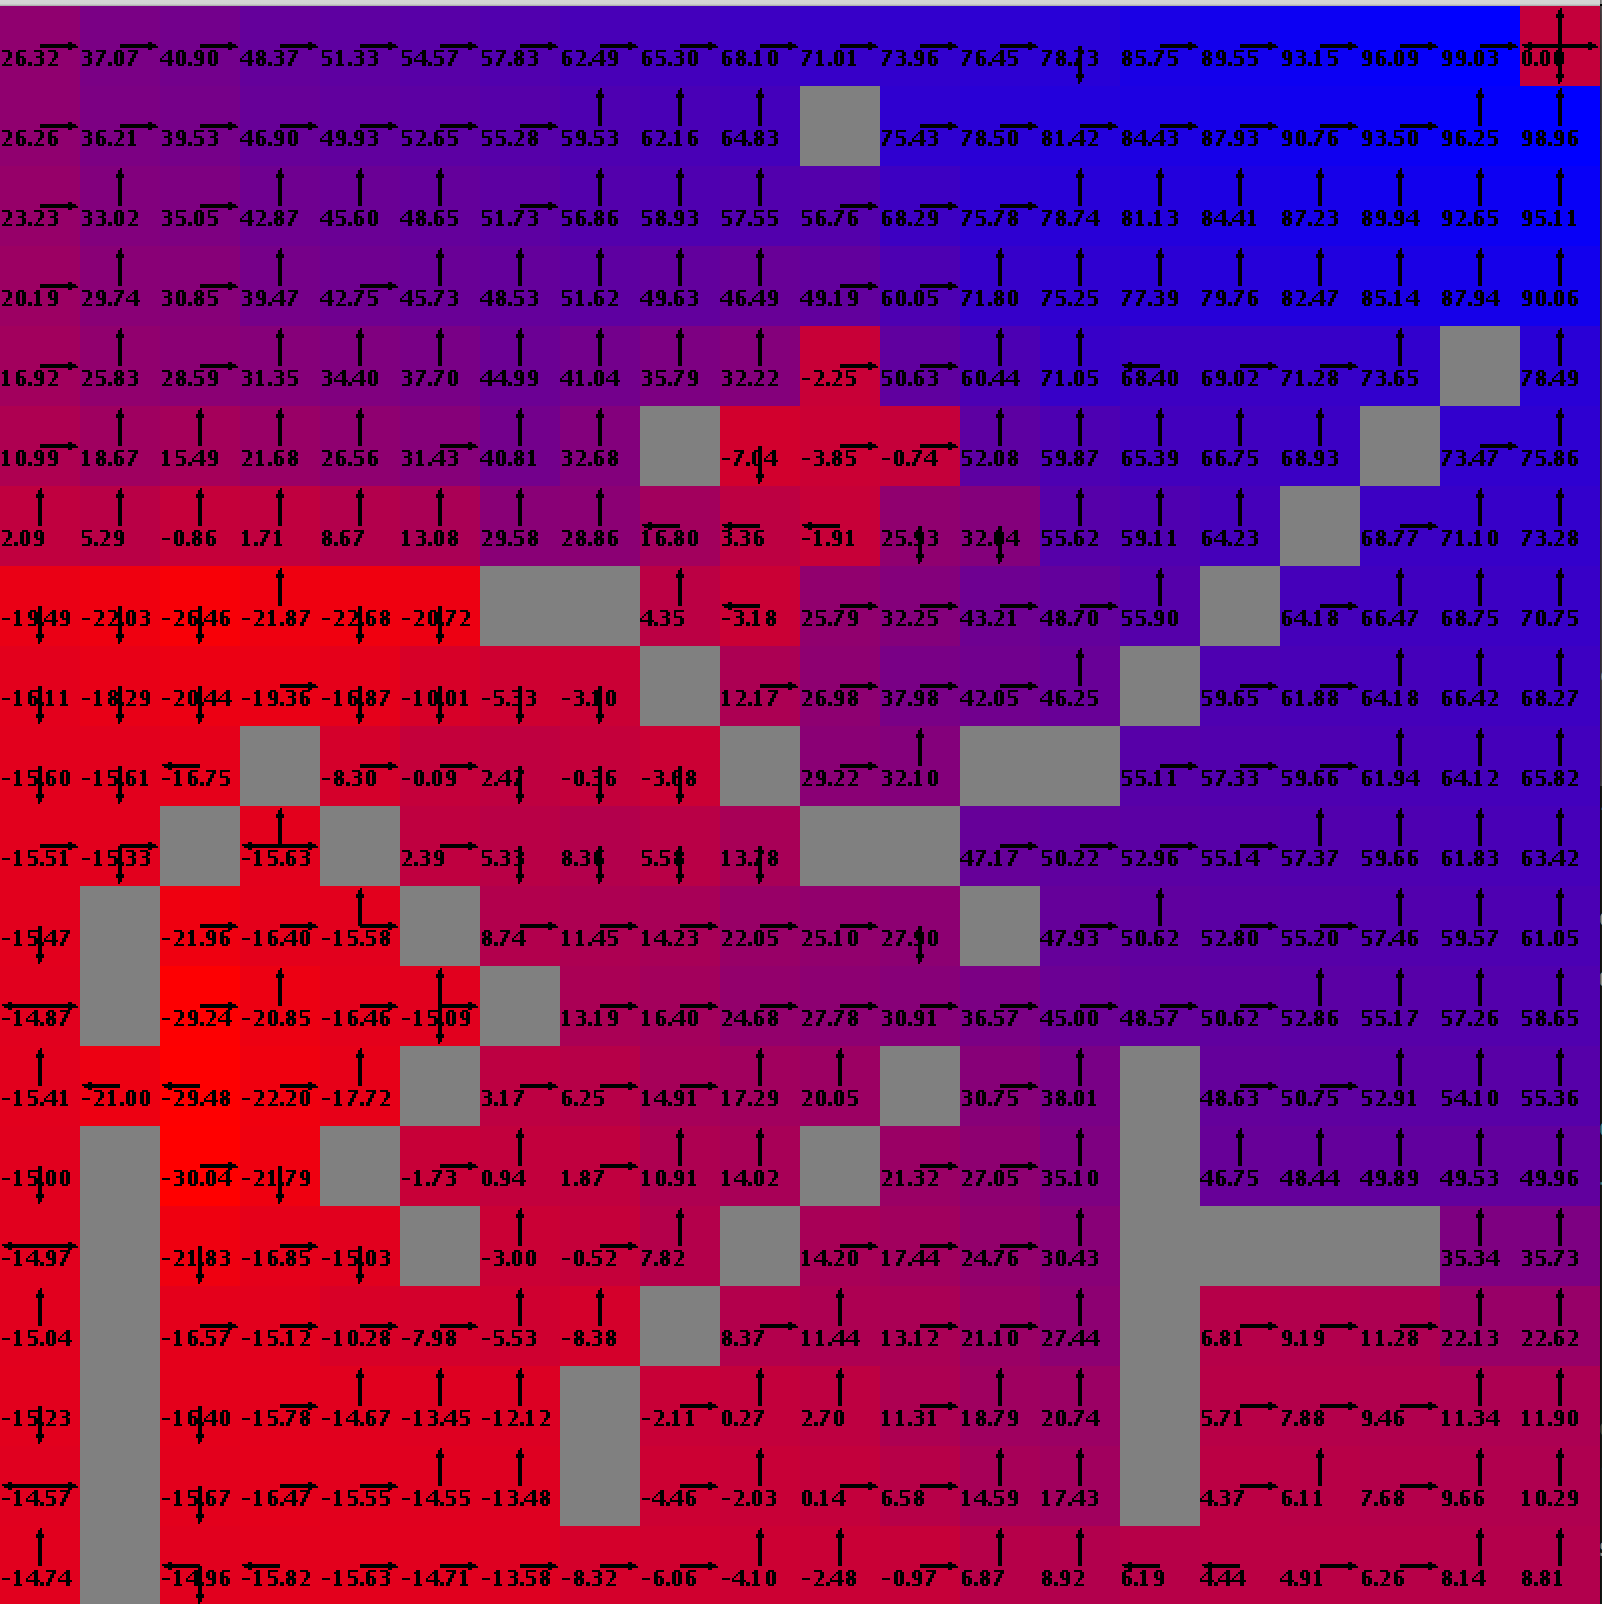
\includegraphics[width=1\textwidth,keepaspectratio]{hard-value-15.png} 
      \caption*{Hard GW Value Iteration \#15} 
   \endminipage\hfill
   \minipage{0.245\textwidth}
      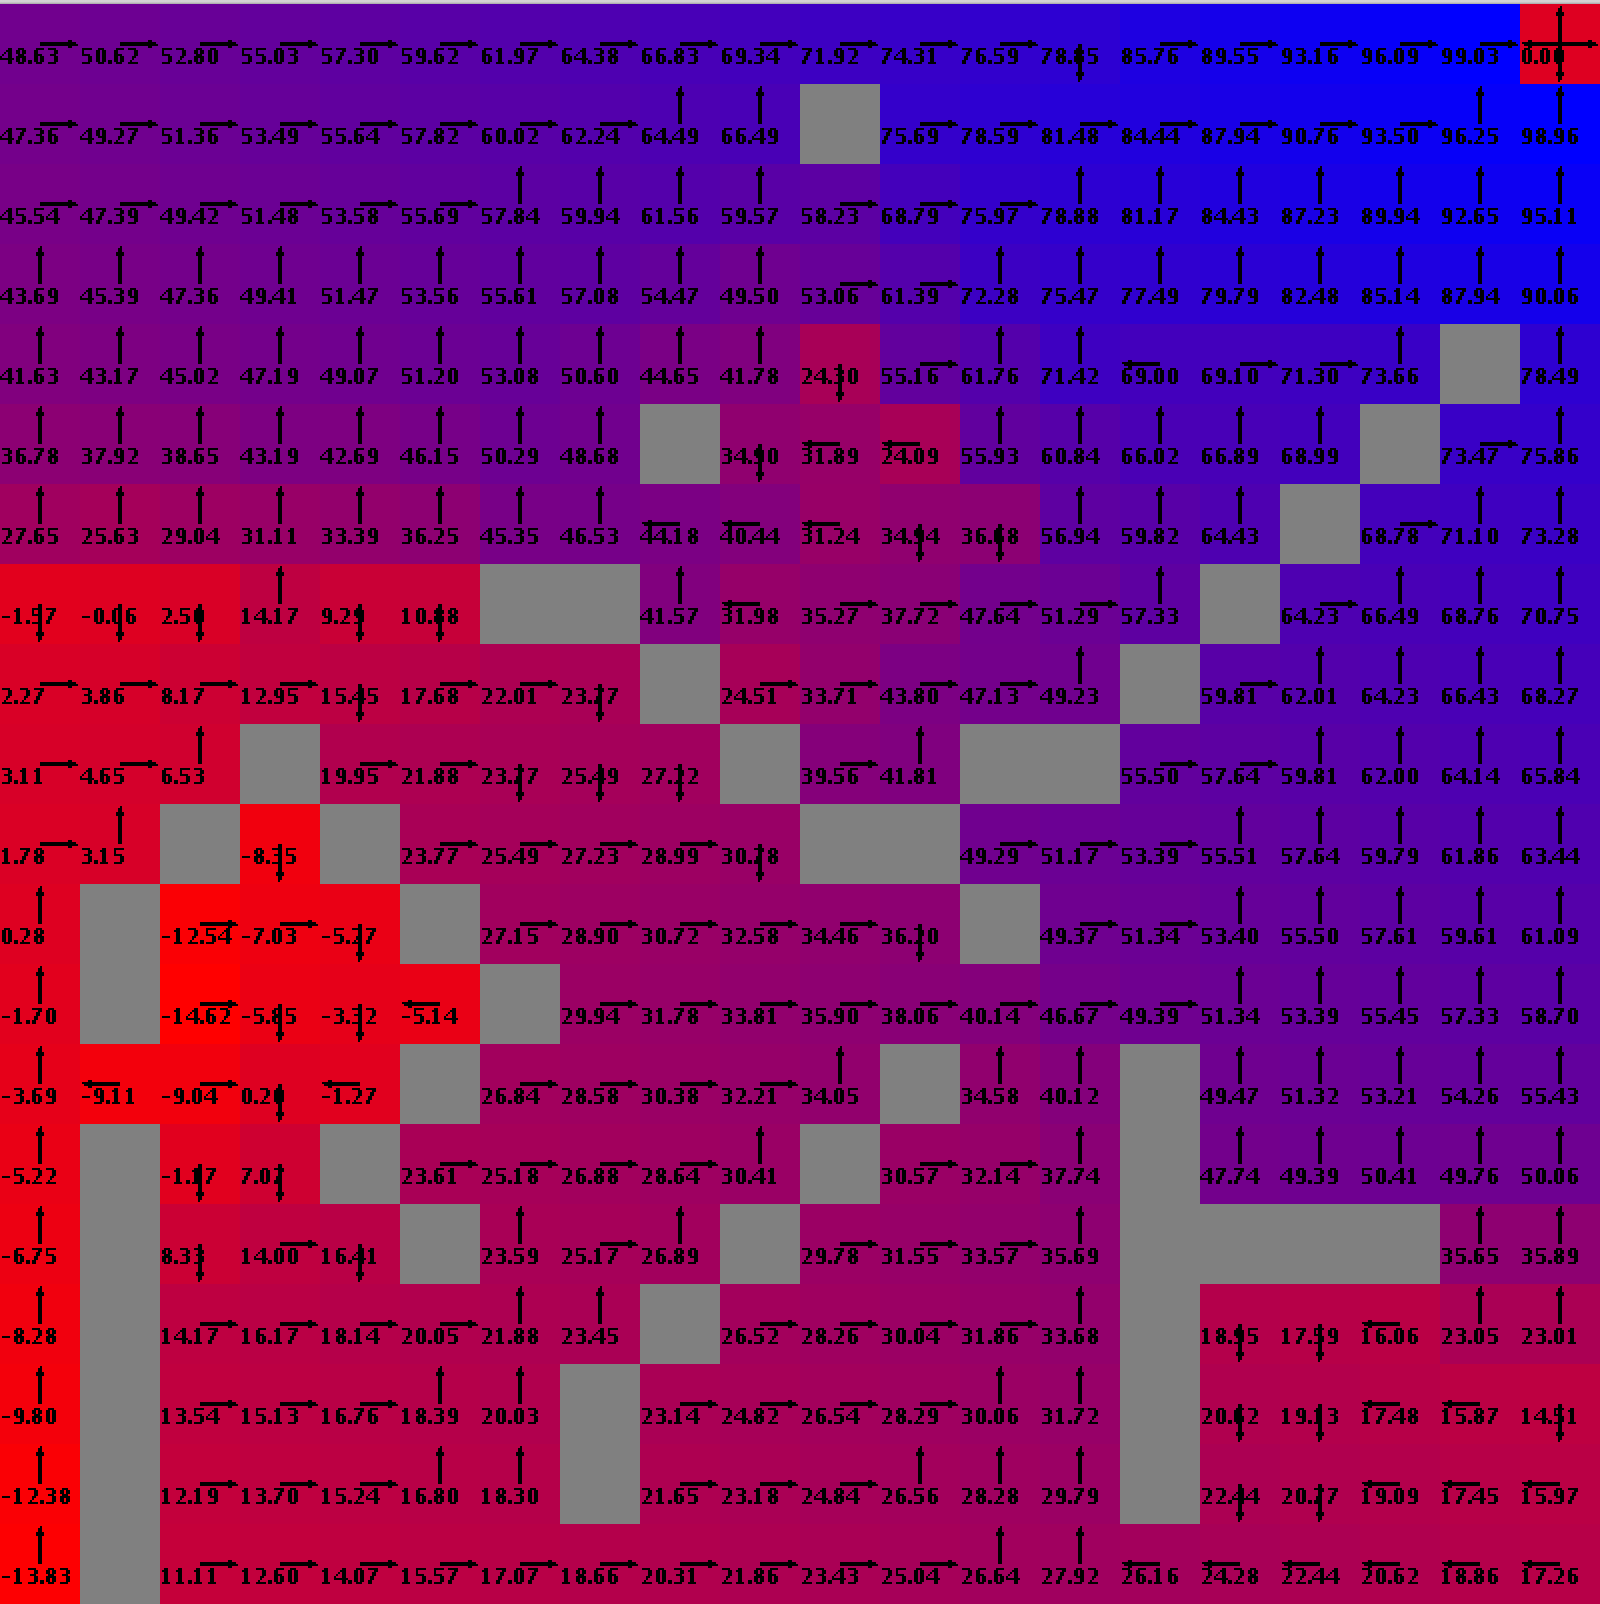
\includegraphics[width=1\textwidth,keepaspectratio]{hard-value-30.png} 
      \caption*{Hard GW Value Iteration \#30} 
   \endminipage\hfill
   \minipage{0.245\textwidth}
      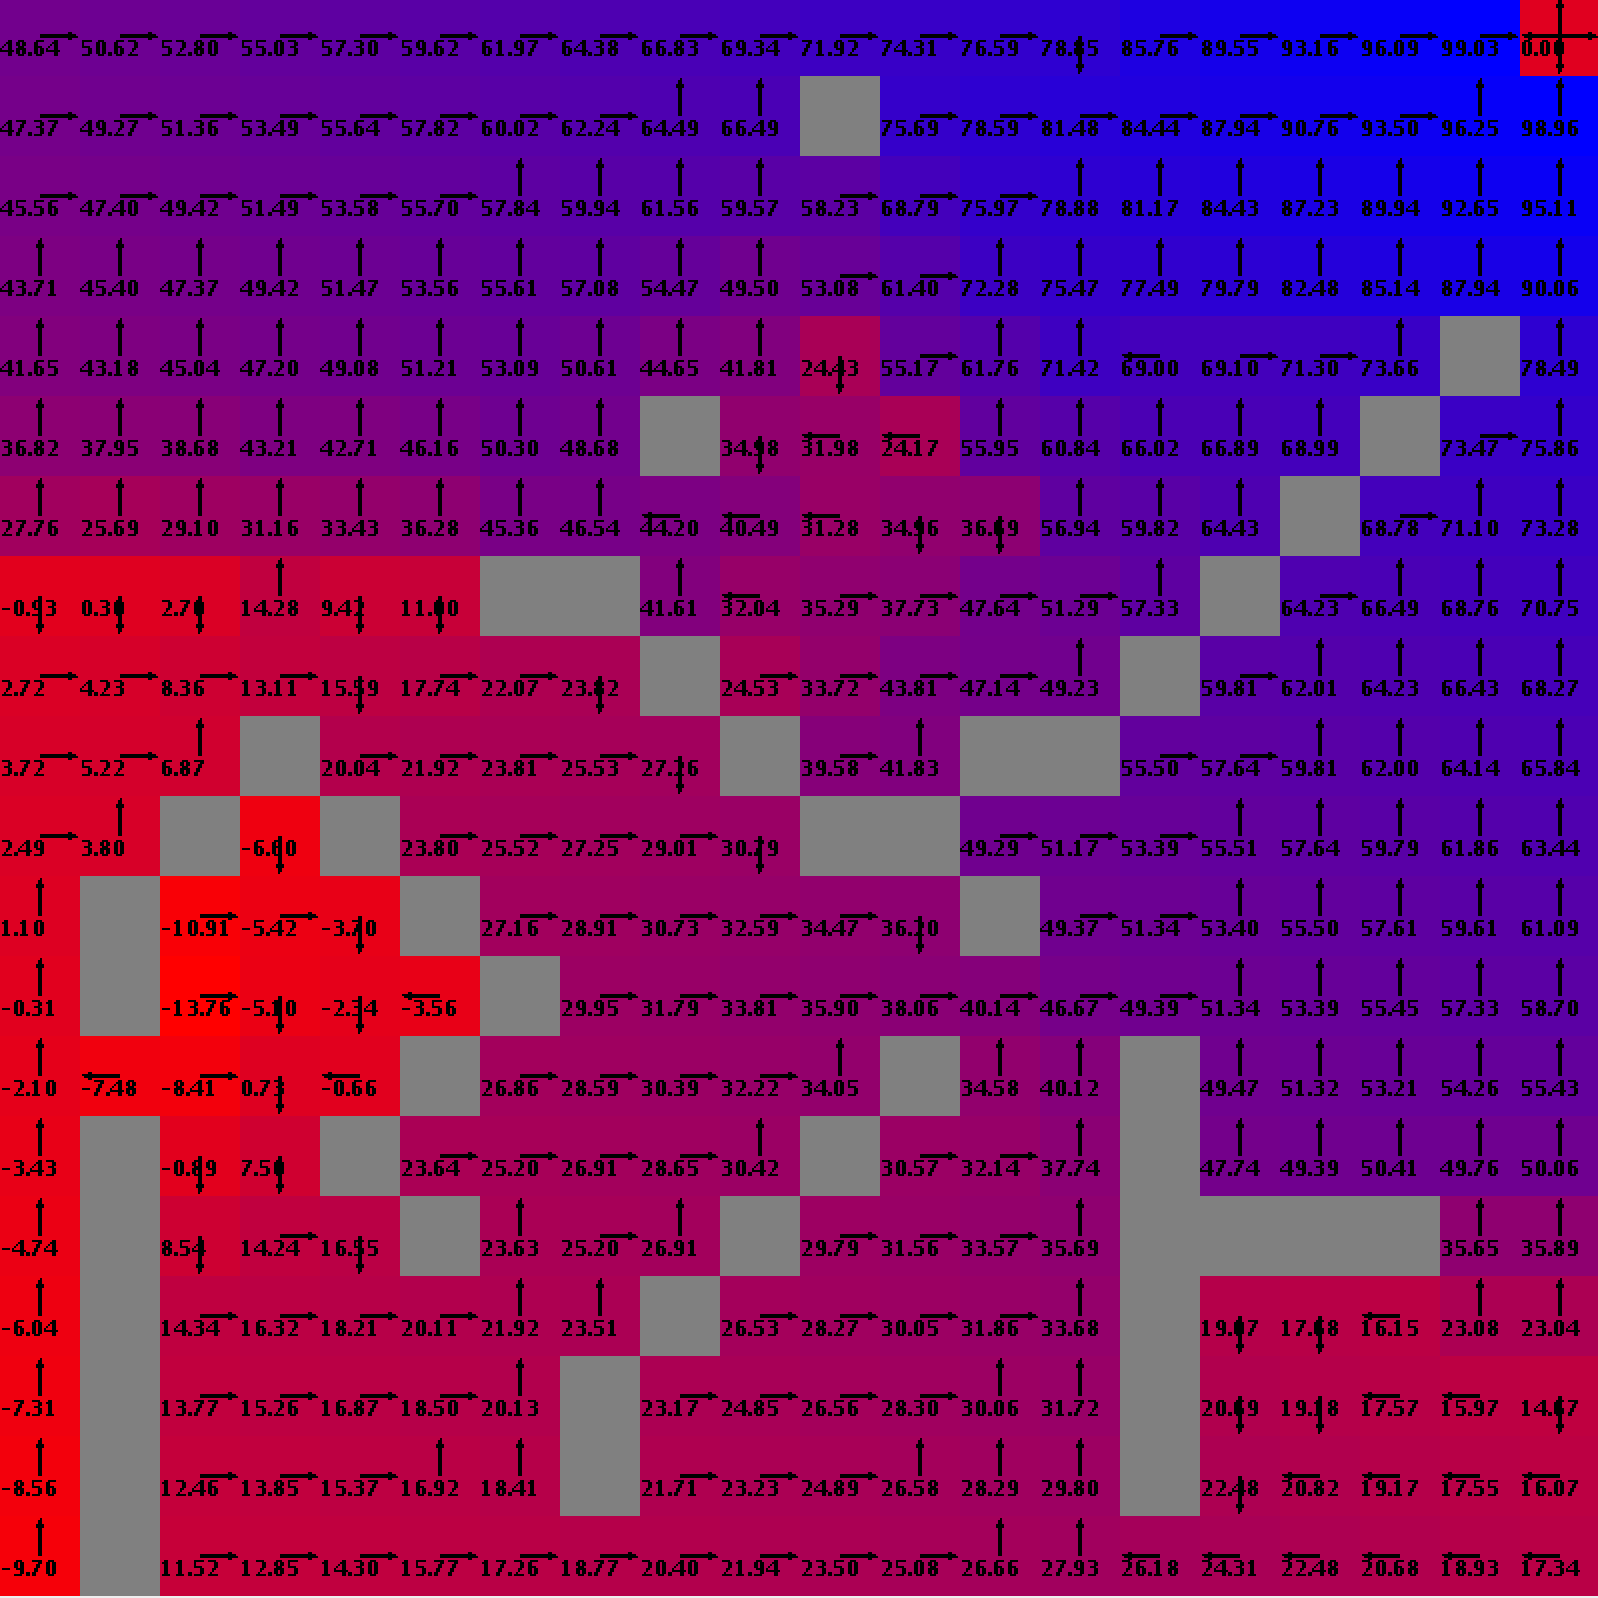
\includegraphics[width=1\textwidth,keepaspectratio]{hard-value-61.png} 
      \caption*{Hard GW Value Iteration \#61} 
   \endminipage\hfill
\end{figure}

 
\section*{Policy Iteration}
\subsection*{Introduction}
The second reinforcement learning algorithm used to optimally solve the MDPs is 
Policy Iteration.  Policy iteration works by beginning with a random policy and then 
attemping to modify it state by state by taking different actions.  This continues throughout each state of the policy in an attempt
 to find a better solution.  When no further policy changes are found, the algorithm 
 is finished.  Policy Iteration tends to take longer than Value Iteration due to 
 the additional number of explorations and calculations being done.
 
  \begin{figure}[H] 
\centering
\begin{tabular}{ | c | c  | c | c | c | c | c | c| c| c| c| c| c | } 
\hline
\textbf{Iterations} & \textbf{Time} & \textbf{Reward} & \textbf{Steps} & \textbf{Convergence}   \\
\hline
\textbf{EASY Gridworld} \\ \hline
1 & 0.0194 & -186.5000 & 190.9400 & 79.8000 \\ \hline
5 & 0.1096 & 43.1000 & 25.2600 & 22.2546 \\ \hline
10 & 0.2077 & 45.2200 & 49.3200 & 3.0887 \\ \hline
15 & 0.2406 & 44.0200 & 48.4200 & 0.0007 \\ \hline
20 & 0.2568 & 44.8400 & 50.6800 & 0.0002 \\ \hline
25 & 0.2747 & 46.0200 & 45.9800 & 1.58e-5 \\ \hline
30 & 0.2907 & 46.7800 & 48.4800 & 2.19e-6 \\ \hline
33 & 0.3021 & 47.9400 & 45.5800 & 8.23e-7 \\ \hline
\\
\textbf{HARD Gridworld} \\ \hline
1 & 0.3033 & -299 & 300 & 83.8936 \\ \hline
5 & 0.9030 & -258.4100 & 267.2600 & 60.8785 \\ \hline
10 & 1.6424 & 10.9300 & 63.3000 & 39.2628 \\ \hline
15 & 2.2504 & 11.5600 & 63.1000 & 1.5369 \\ \hline
20 & 2.4257 & 10.3800 & 64.2100 & 5.11e-6 \\ \hline
22 & 2.4633 & 9.9600 & 64.2300 & 8.07e-7 \\ \hline

\end{tabular}
\caption*{Gridworld Policy Iteration Results} 
\end{figure}
 
    \begin{figure}[H]
  \minipage{0.245\textwidth}
      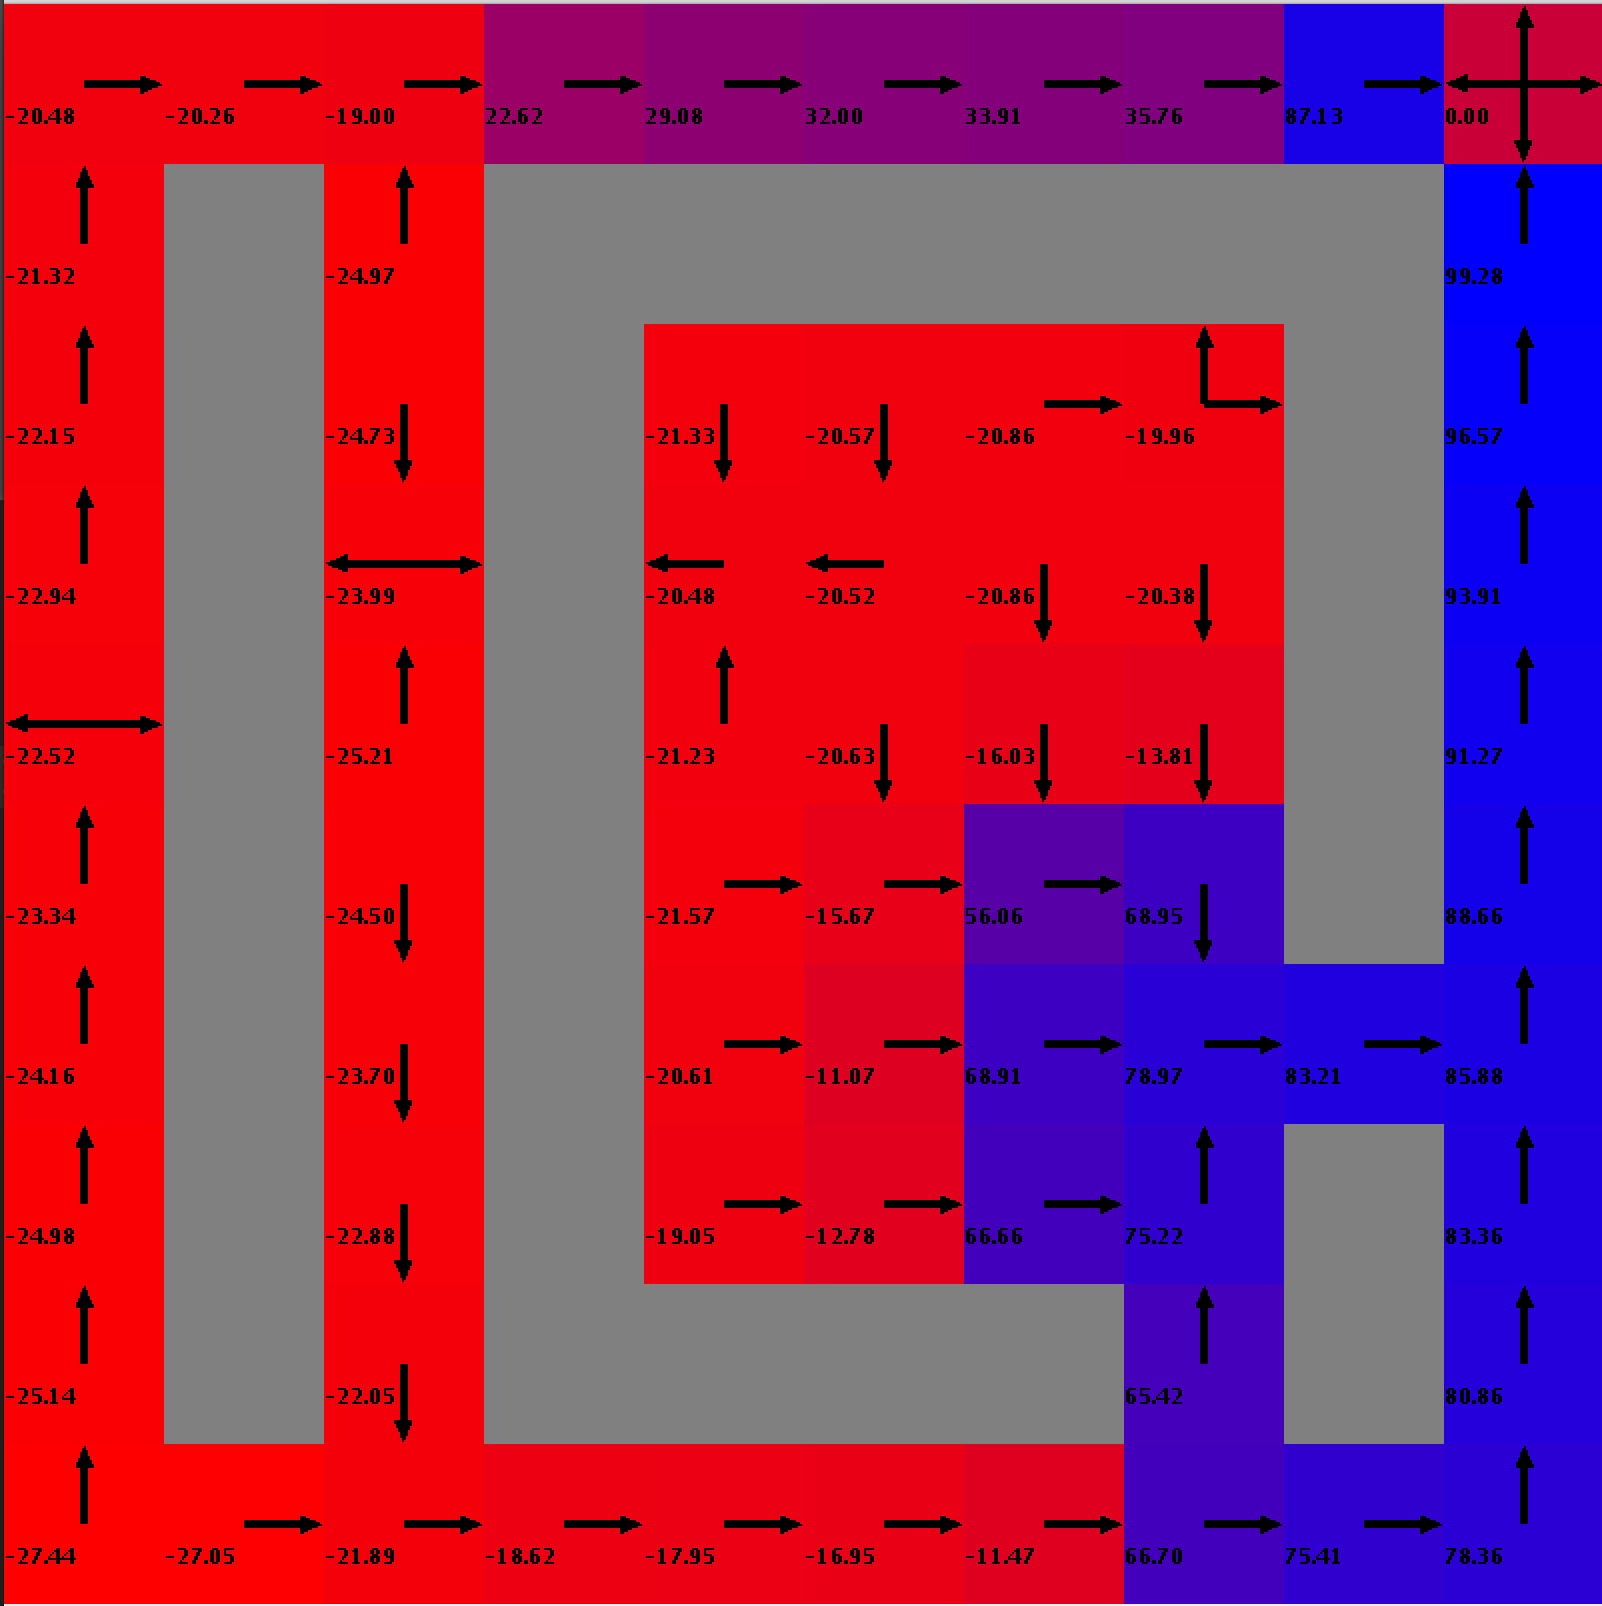
\includegraphics[width=1\textwidth,keepaspectratio]{easy-policy-2.png} 
      \caption*{Easy GW Policy Iteration \#2} 
   \endminipage\hfill
   \minipage{0.245\textwidth}
      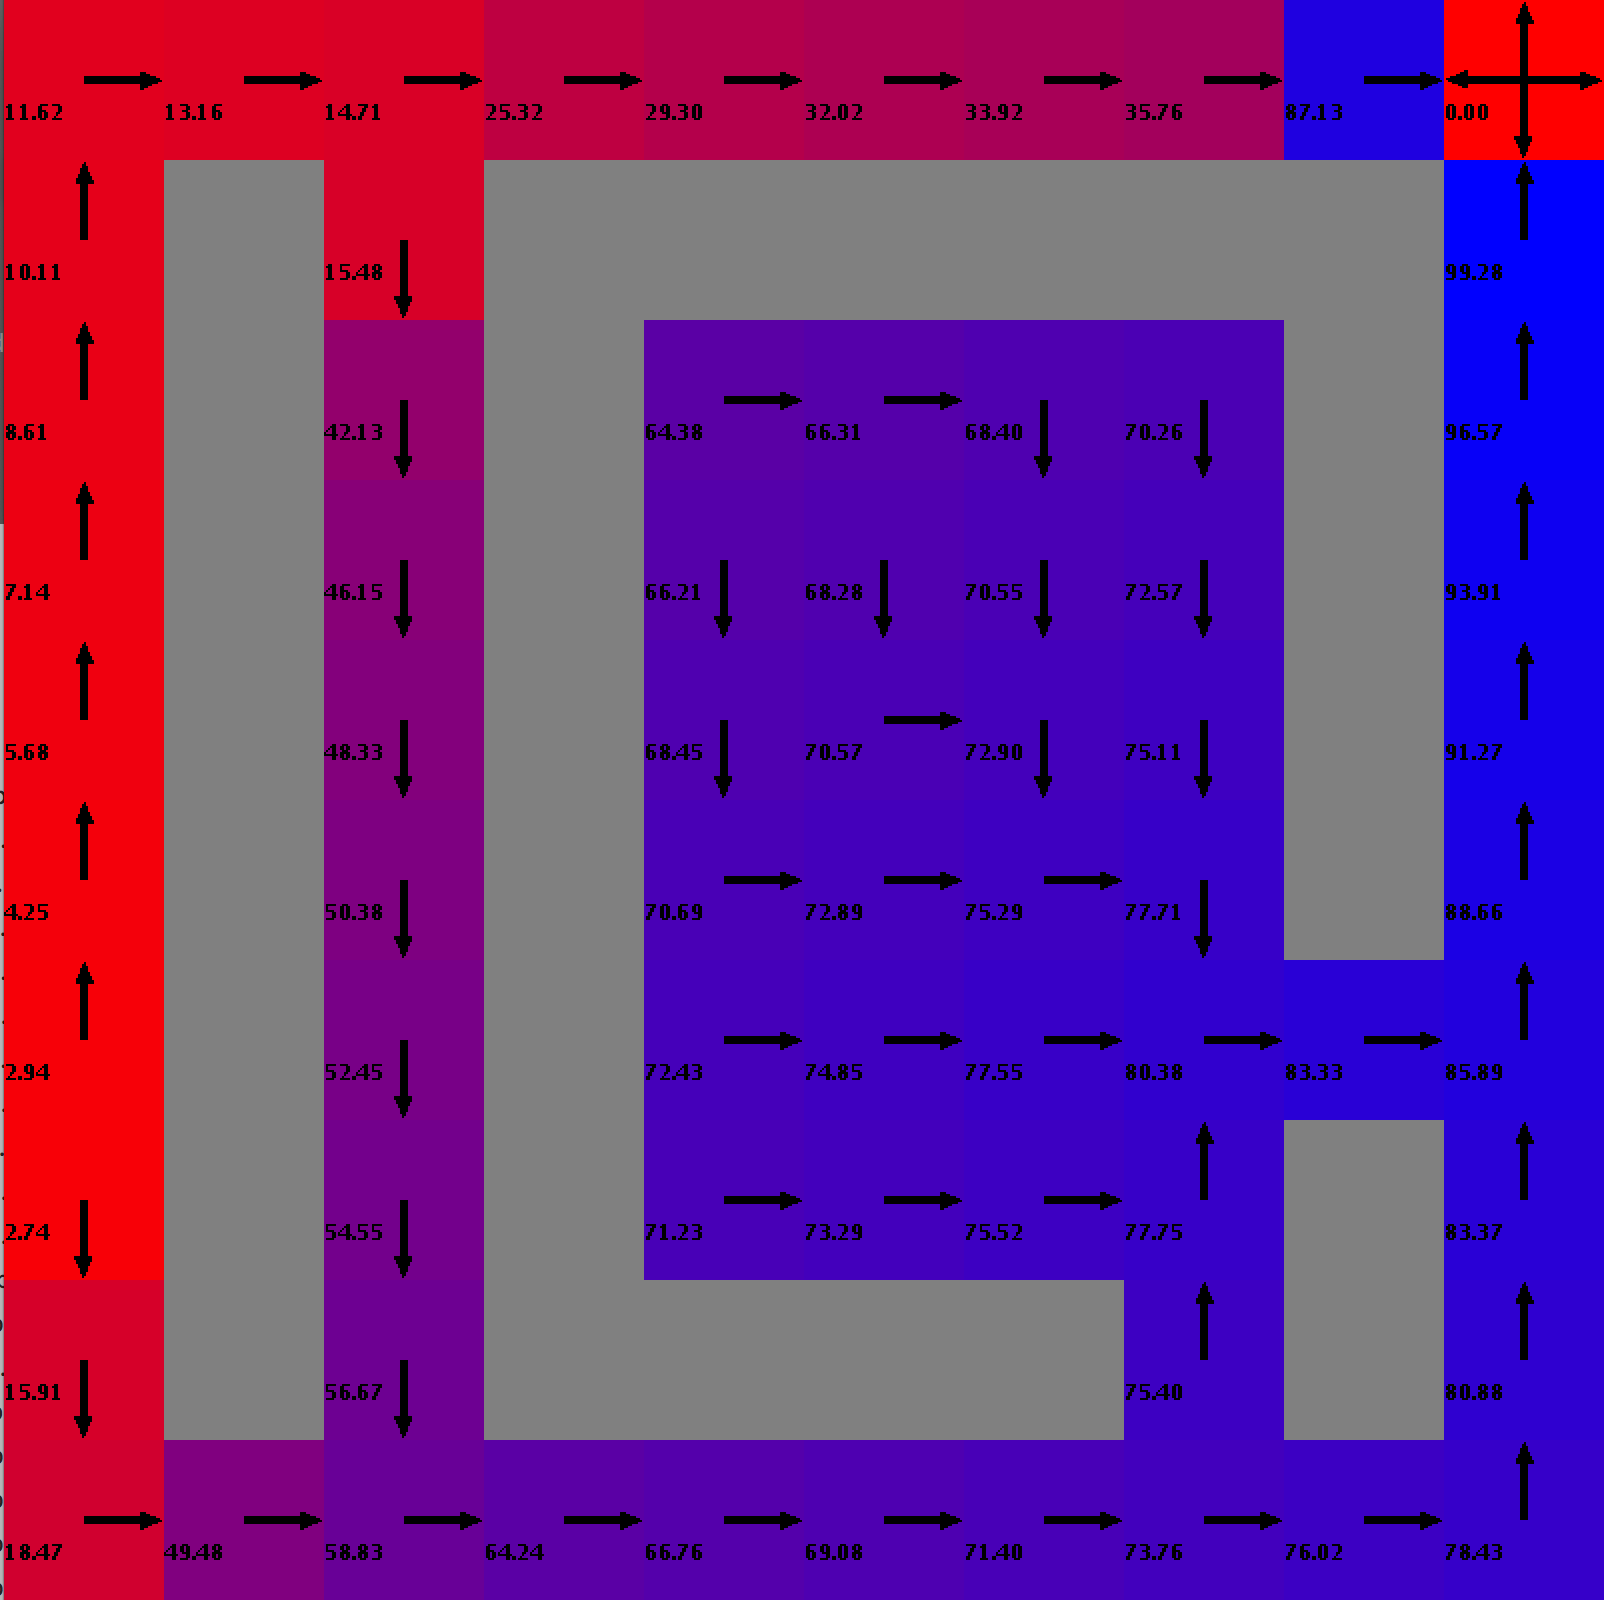
\includegraphics[width=1\textwidth,keepaspectratio]{easy-policy-5.png} 
      \caption*{Easy GW Policy Iteration \#5} 
   \endminipage\hfill
   \minipage{0.245\textwidth}
      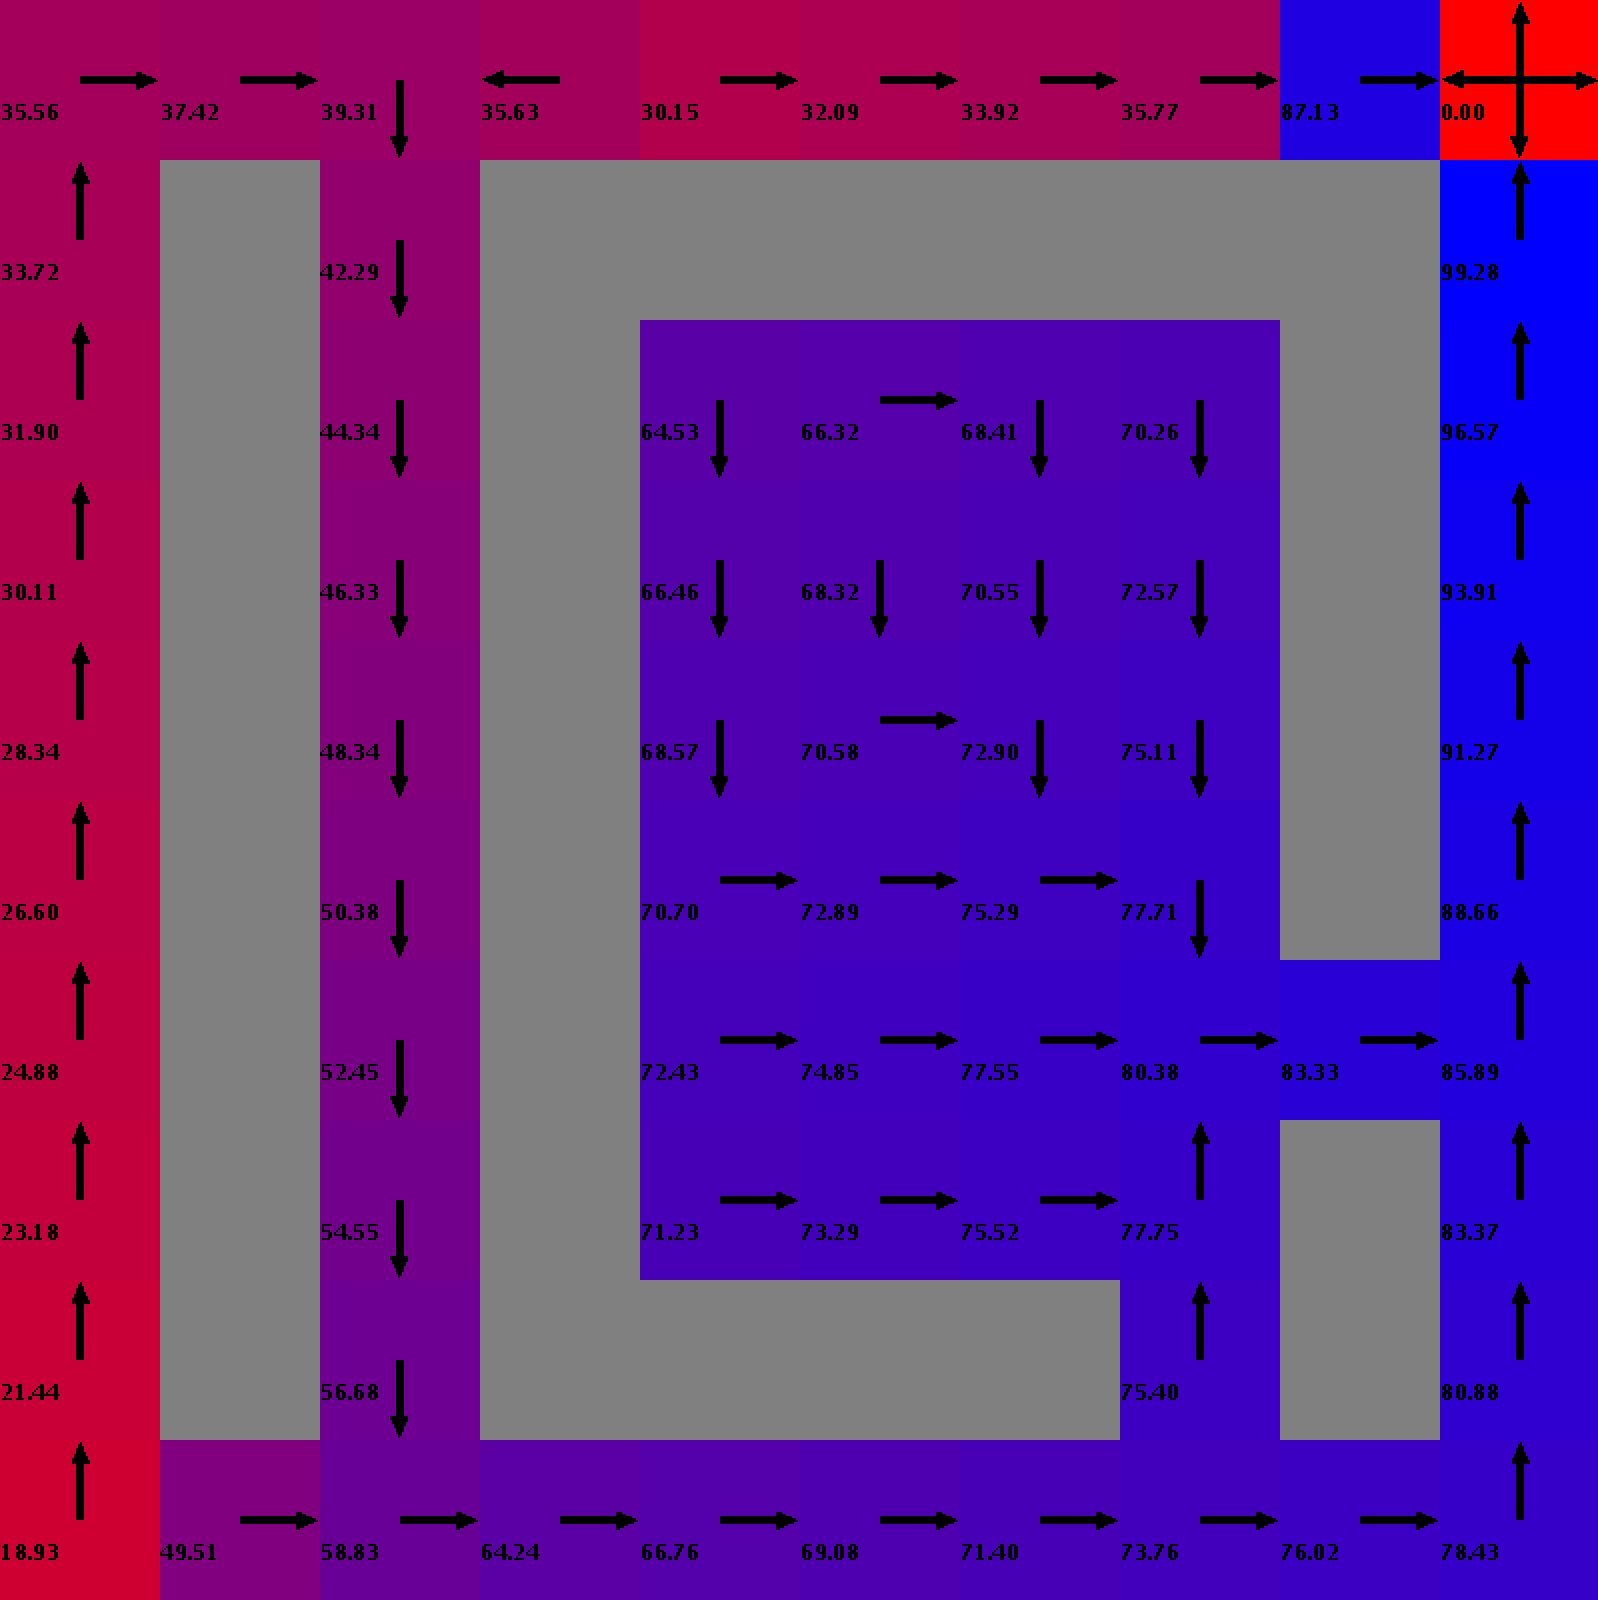
\includegraphics[width=1\textwidth,keepaspectratio]{easy-policy-10.png} 
      \caption*{Easy GW Policy Iteration \#10} 
   \endminipage\hfill
   \minipage{0.245\textwidth}
      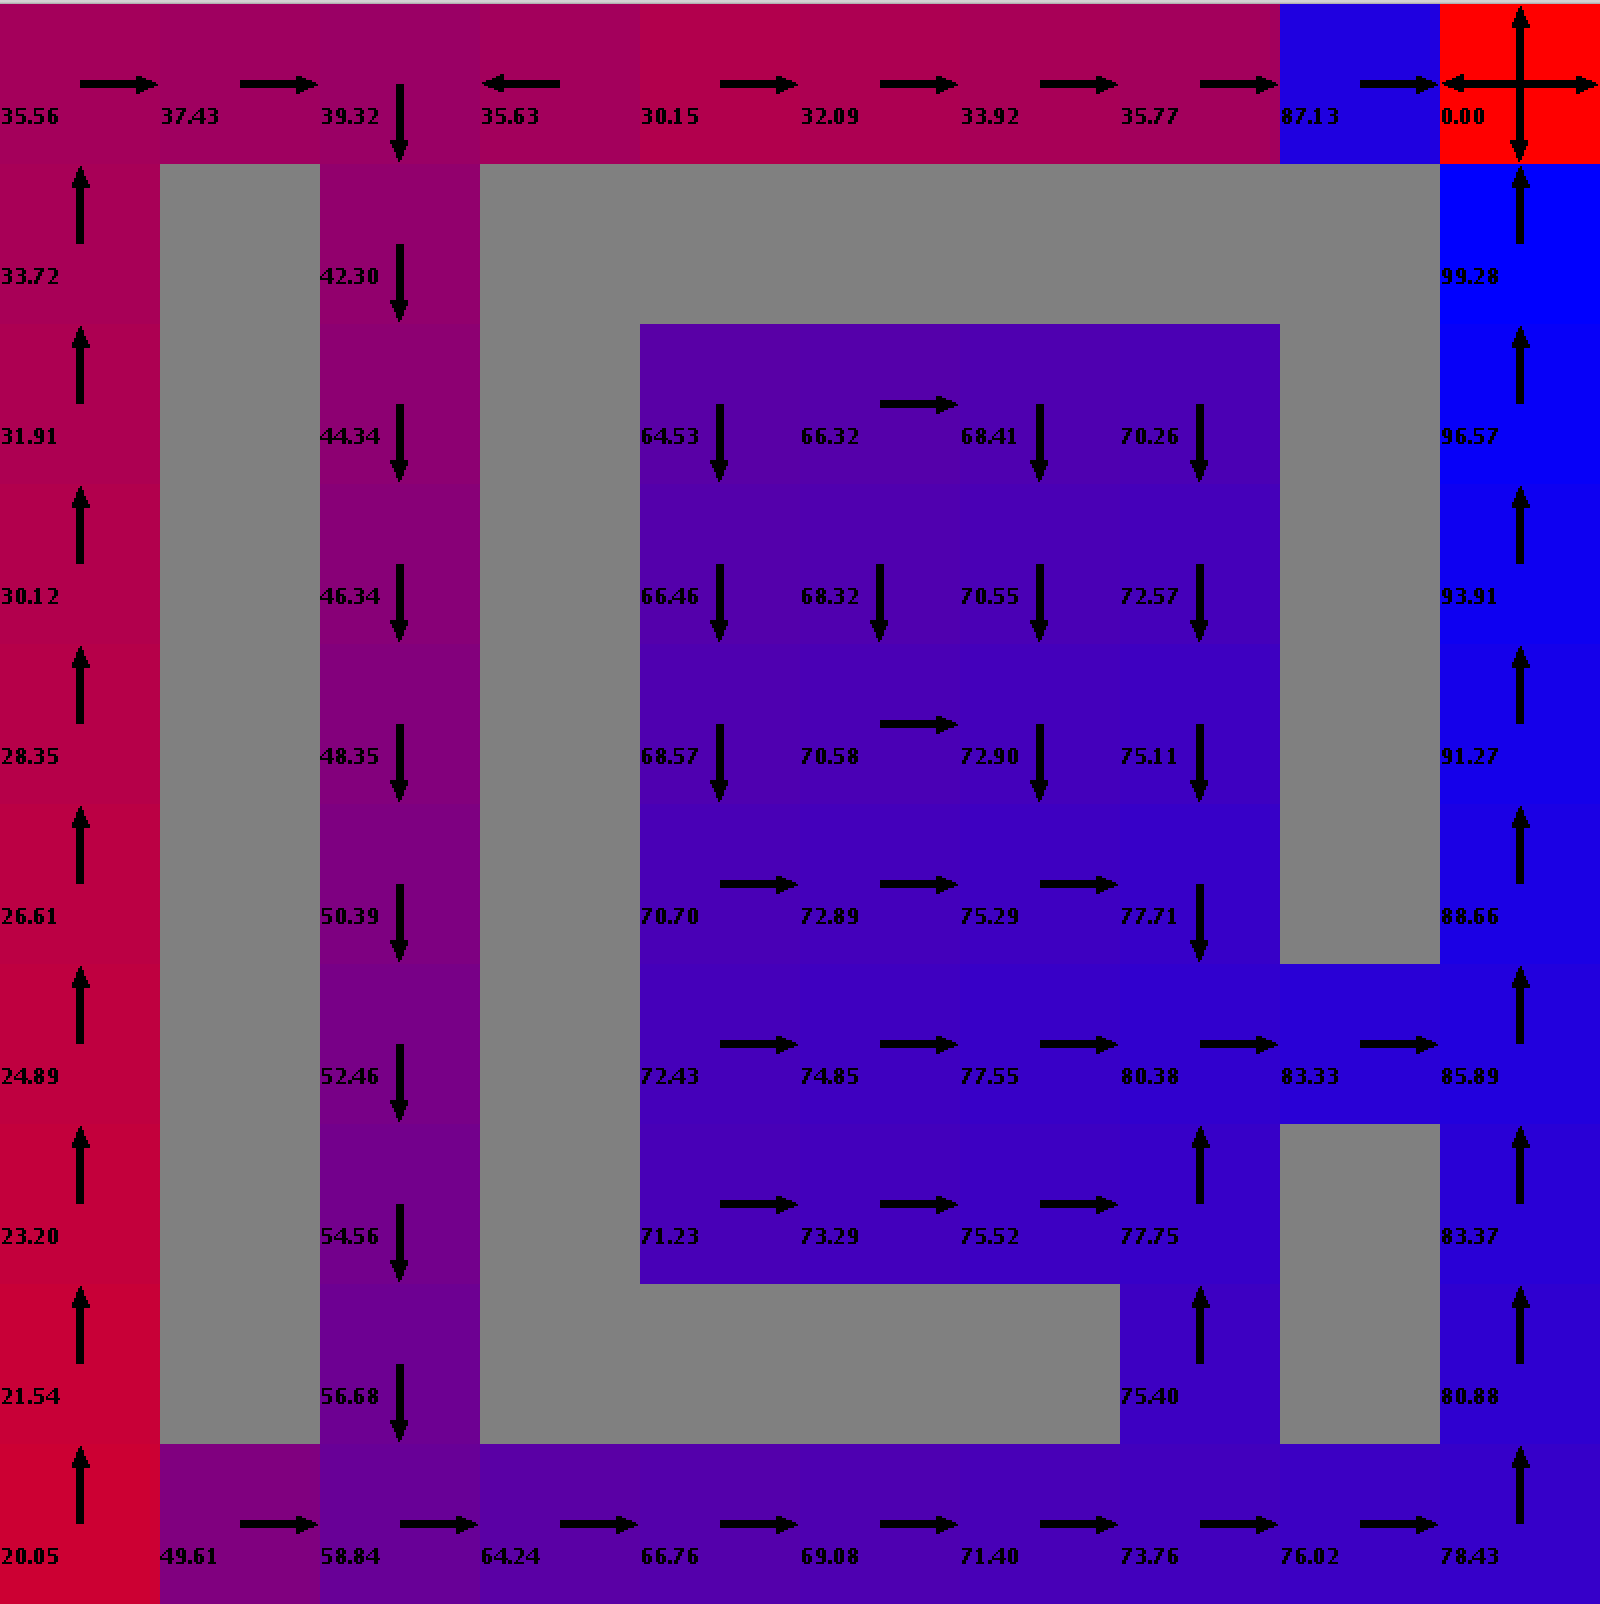
\includegraphics[width=1\textwidth,keepaspectratio]{easy-policy-33.png} 
      \caption*{Easy GW Policy Iteration \#33} 
   \endminipage\hfill
\end{figure}


   \begin{figure}[H]
  \minipage{0.245\textwidth}
      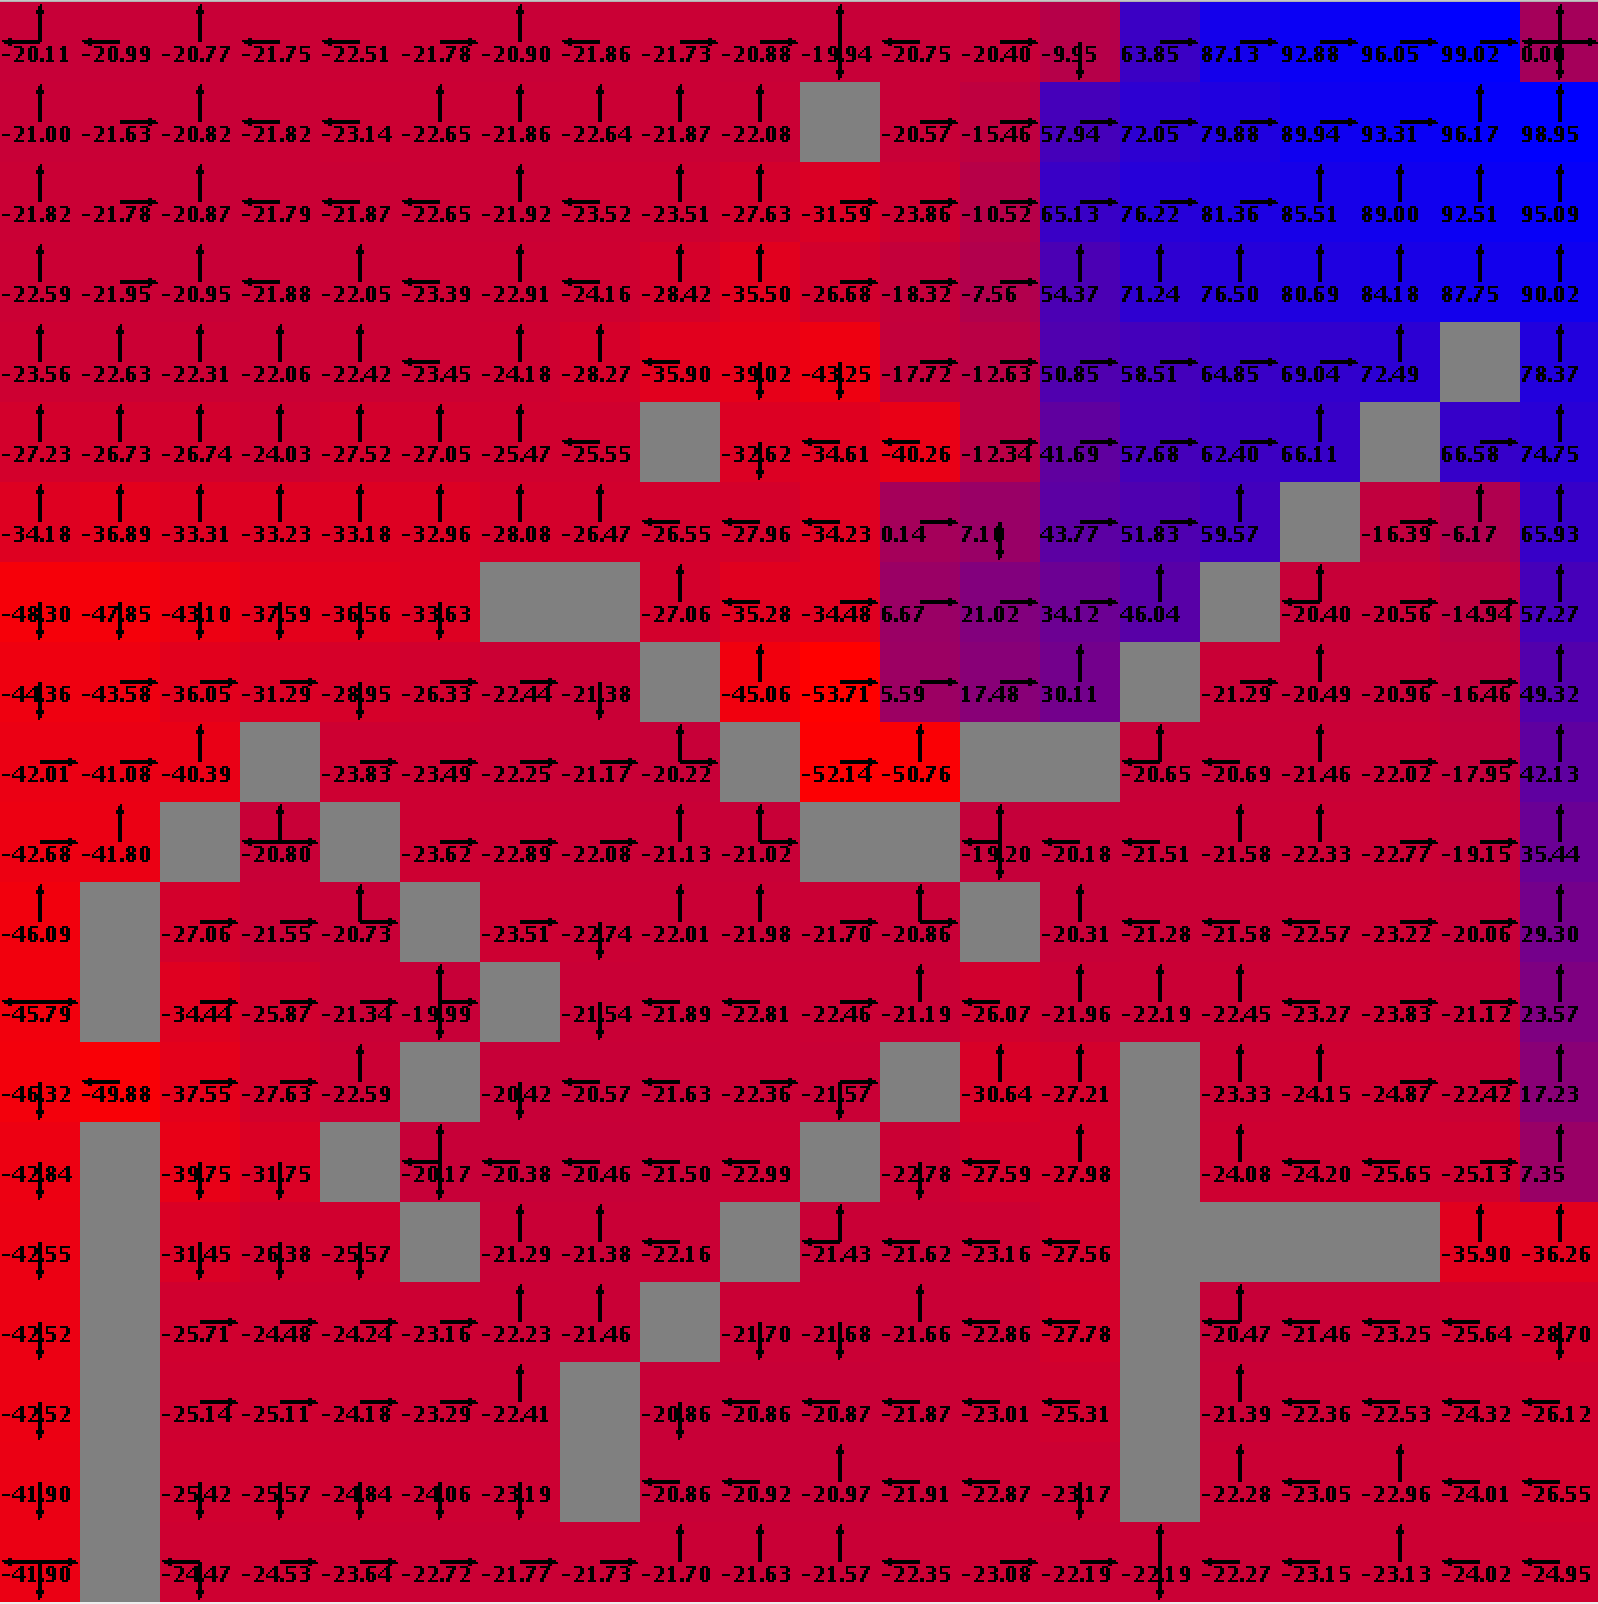
\includegraphics[width=1\textwidth,keepaspectratio]{hard-policy-2.png} 
      \caption*{Hard GW Policy Iteration \#2} 
   \endminipage\hfill
   \minipage{0.245\textwidth}
      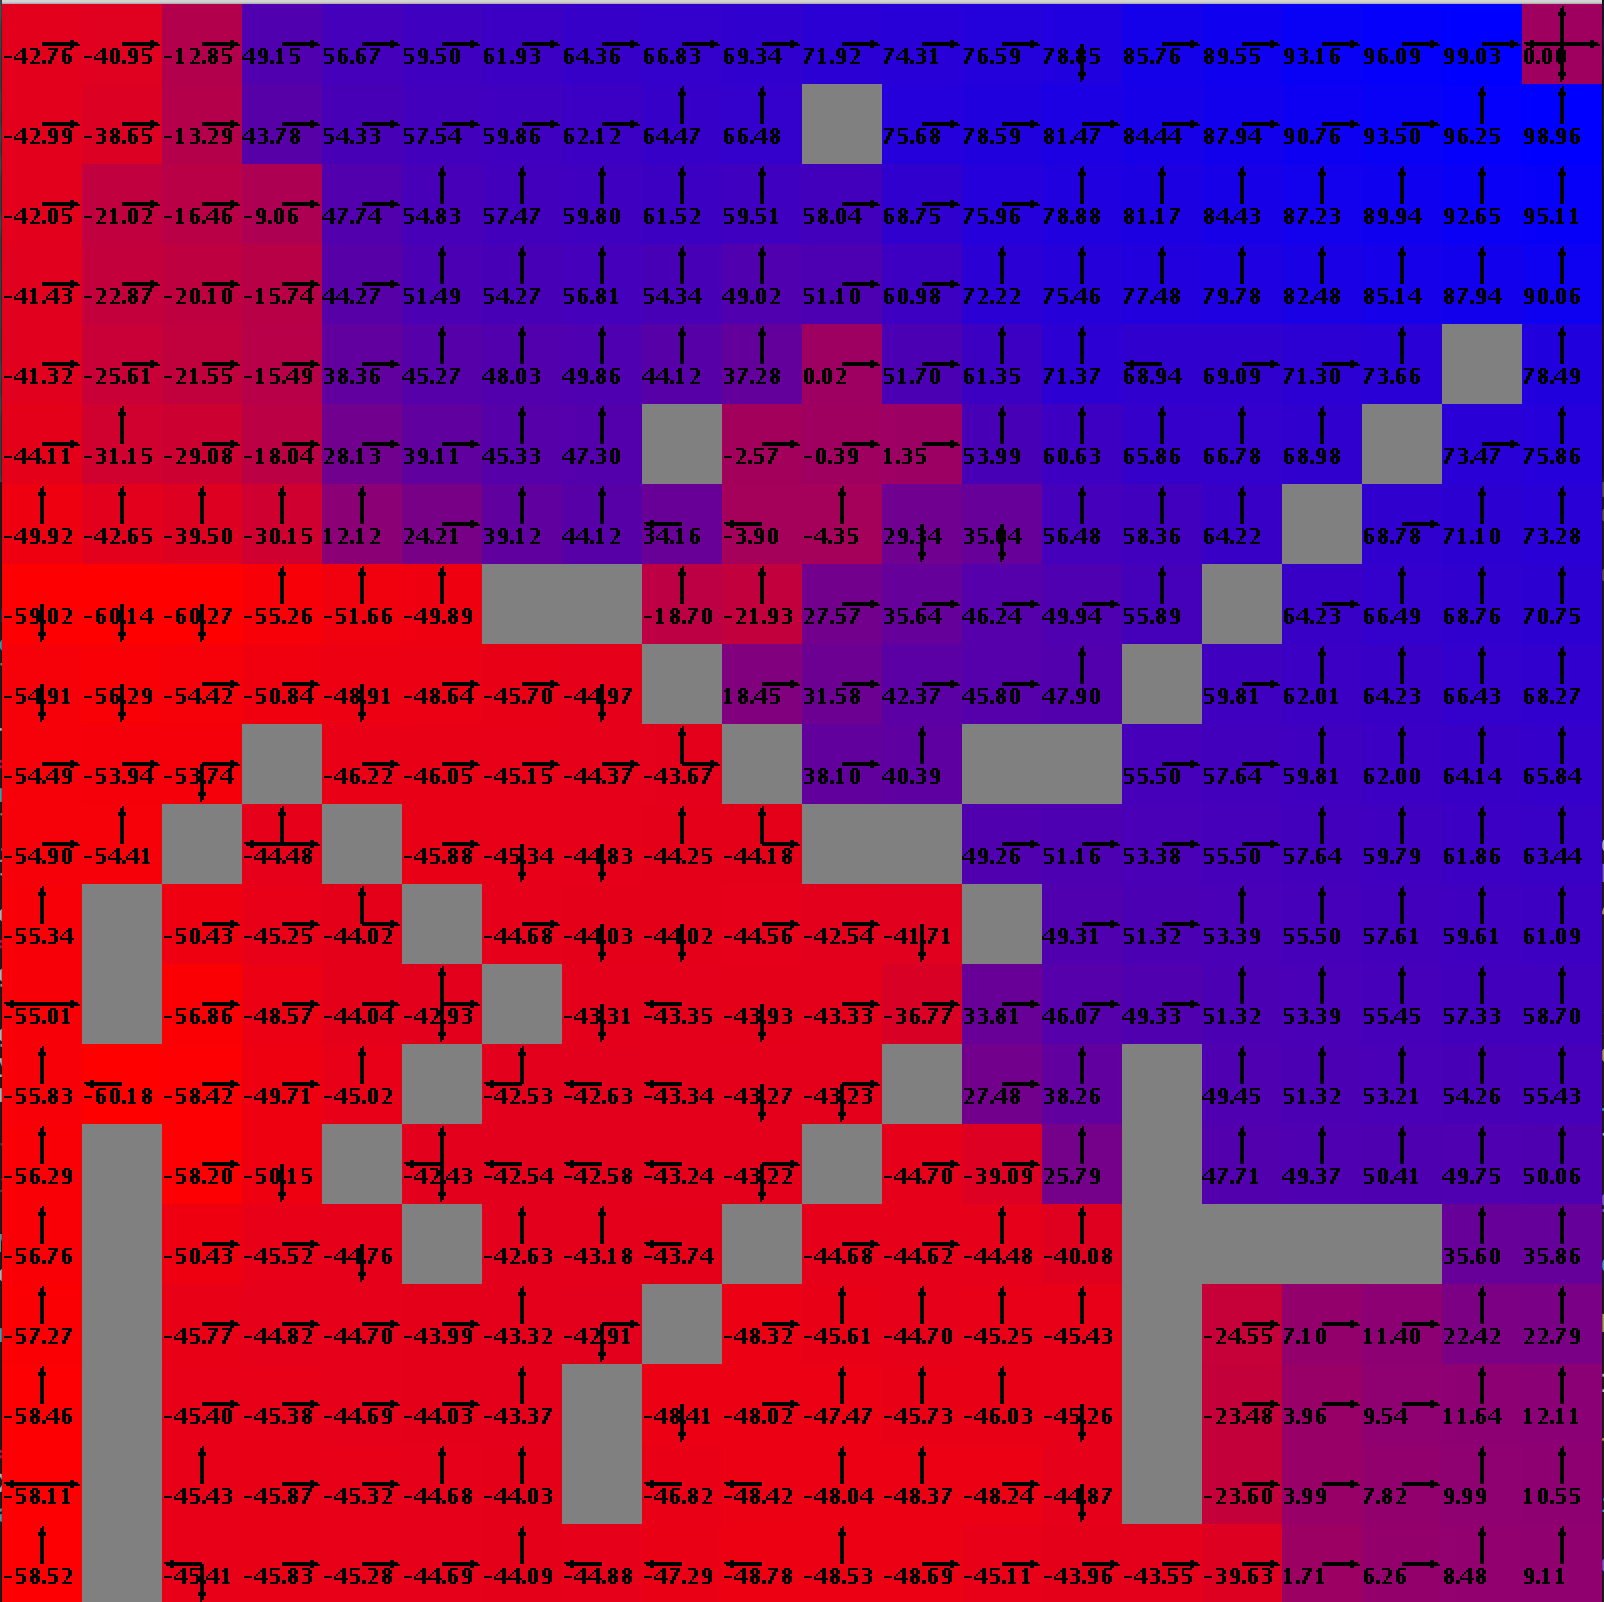
\includegraphics[width=1\textwidth,keepaspectratio]{hard-policy-5.png} 
      \caption*{Hard GW Policy Iteration \#5} 
   \endminipage\hfill
   \minipage{0.245\textwidth}
      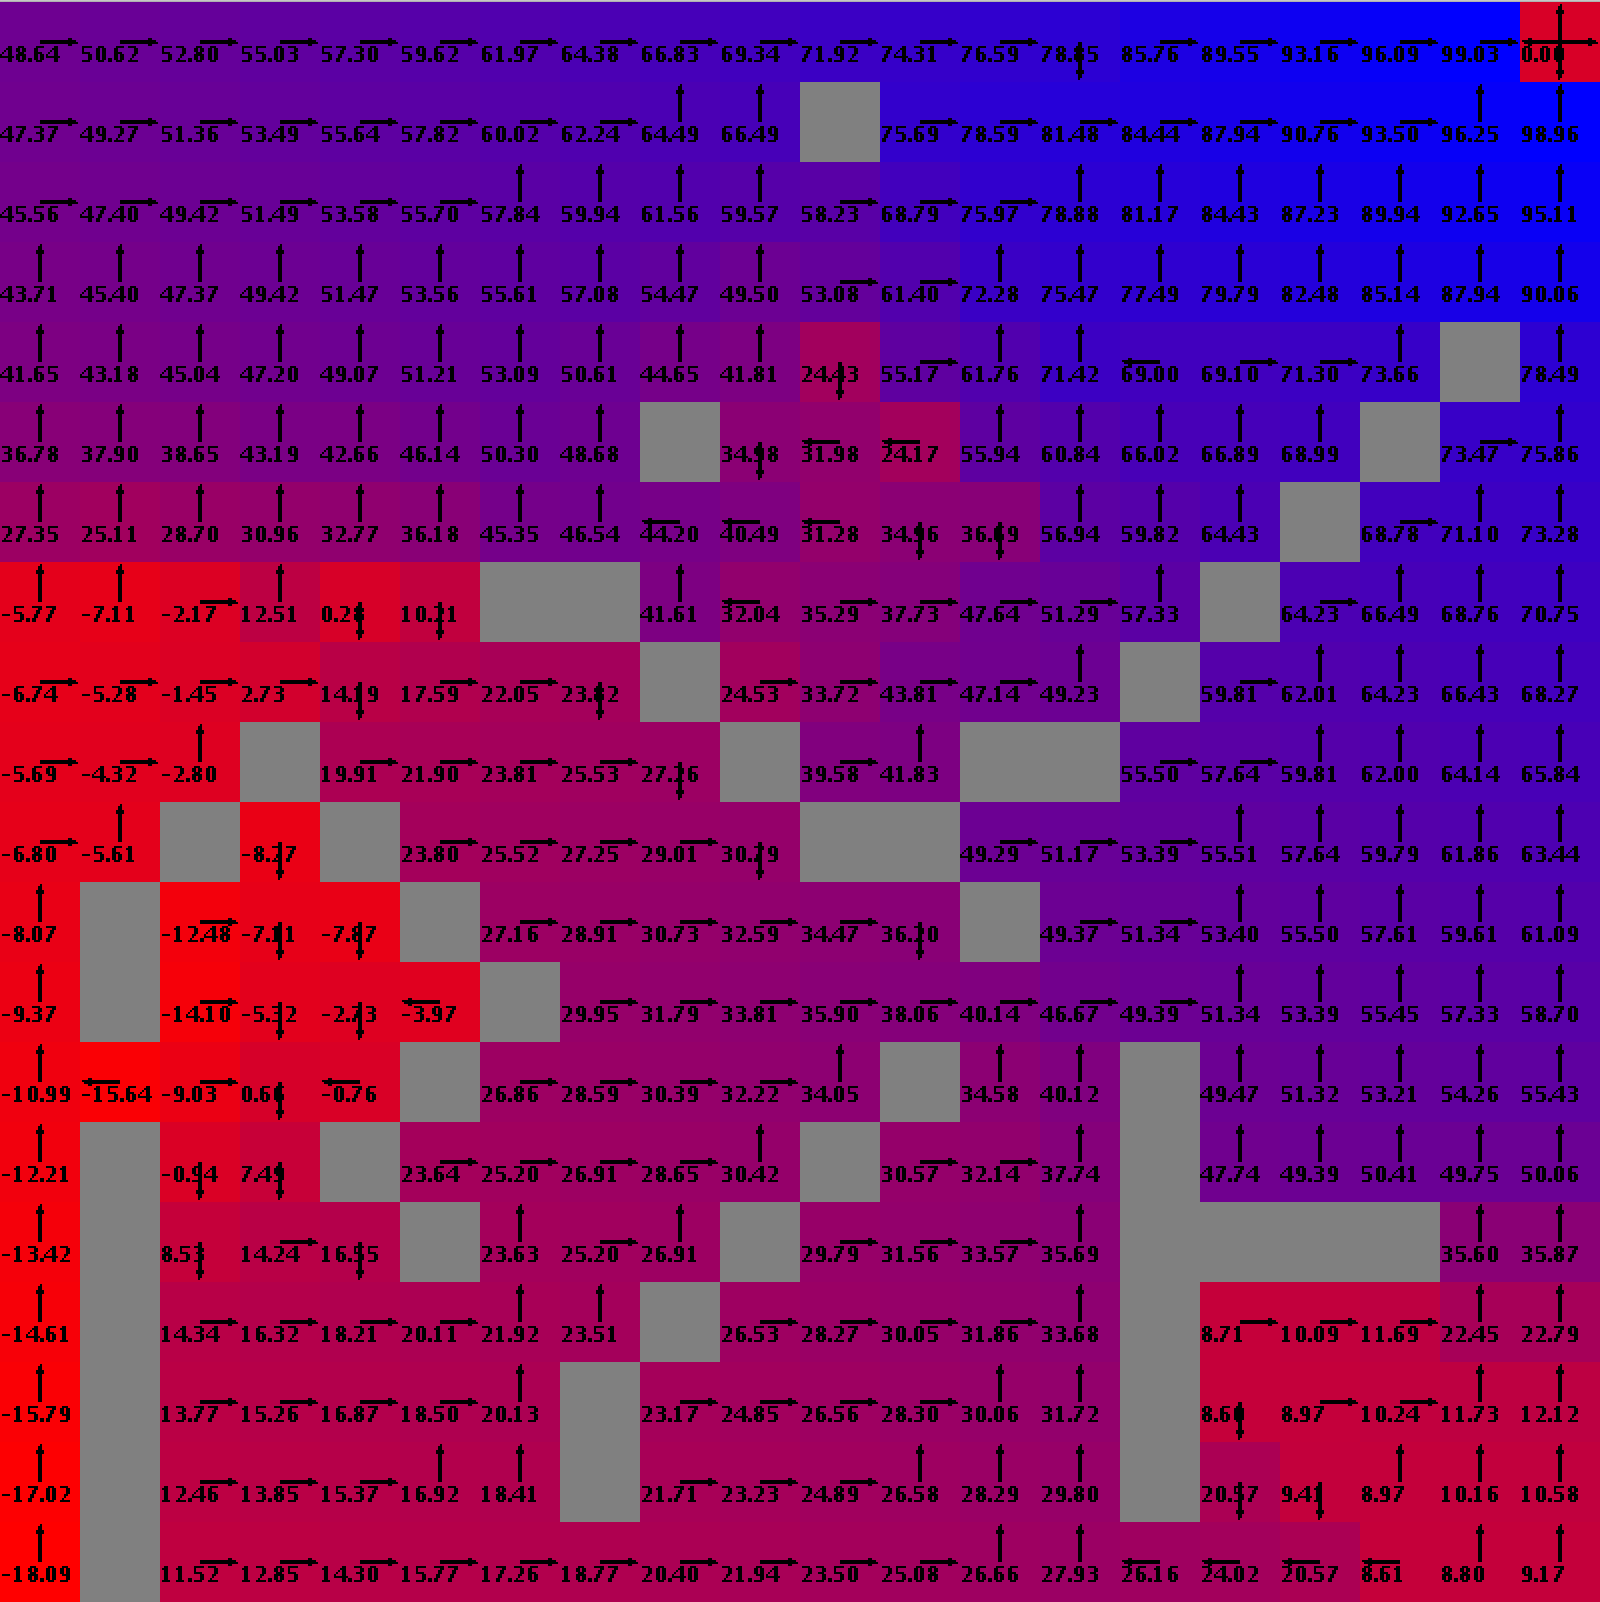
\includegraphics[width=1\textwidth,keepaspectratio]{hard-policy-10.png} 
      \caption*{Hard GW Policy Iteration \#10} 
   \endminipage\hfill
   \minipage{0.245\textwidth}
      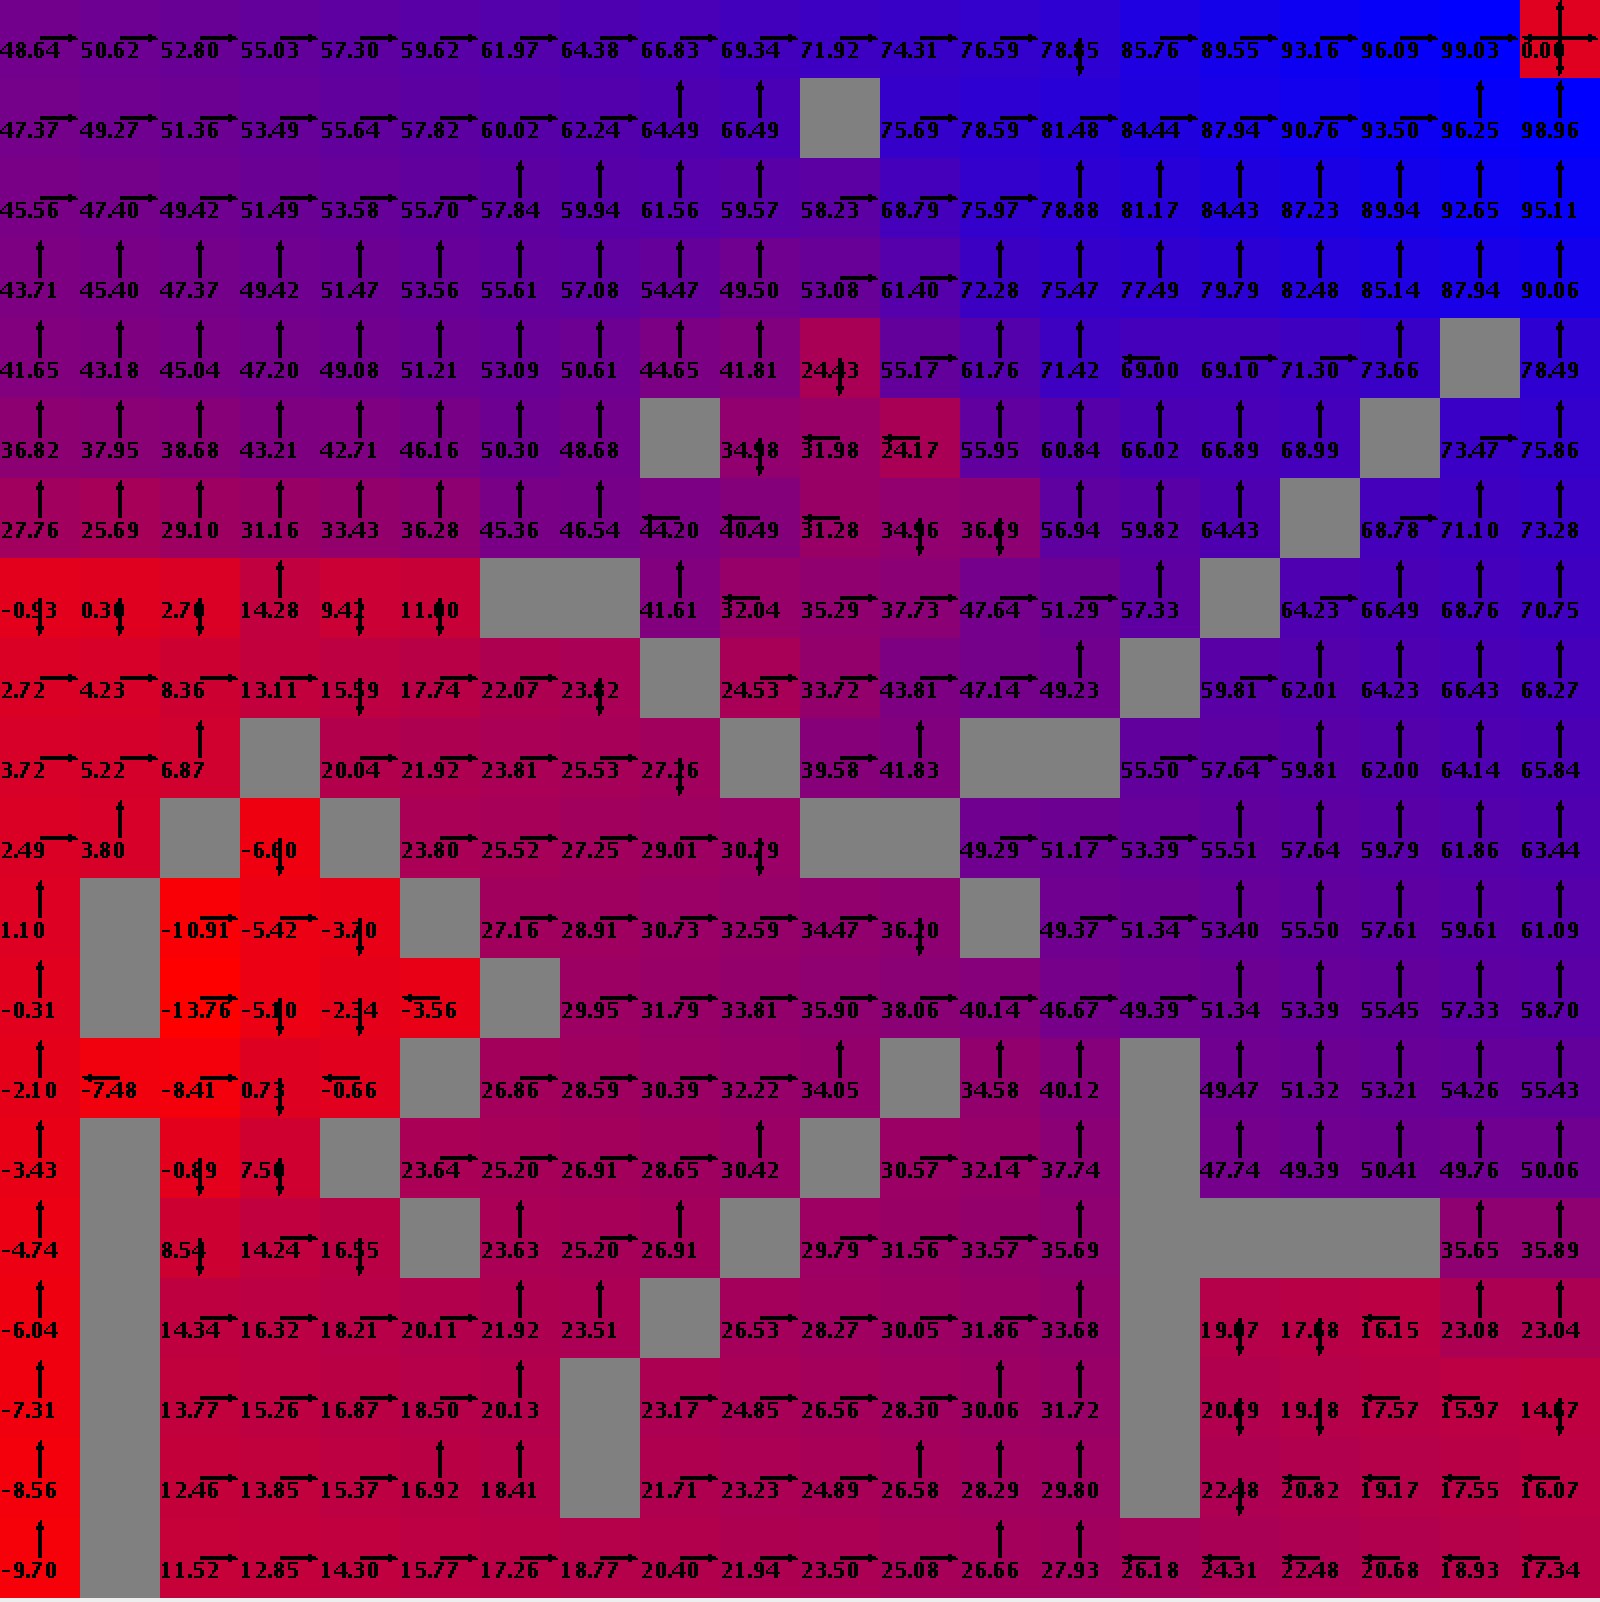
\includegraphics[width=1\textwidth,keepaspectratio]{hard-policy-22.png} 
      \caption*{Hard GW Policy Iteration \#22} 
   \endminipage\hfill
\end{figure}



 
\section*{Q-learning}
\subsection*{Introduction}
The third reinforcement algorithm used to optimally solve the MDPs is 
Q-learning.  Q-learning works by assigning q values to every state.  At each state, the learner calculates new 
q values based on both immediate and future rewards.  Initially, Q-learning will 
spend time exploring and learning, whereas it will eventually optimize
based on knowledge learned and converge.  While the first two algorithms have domain knowledge about the problem, 
Q-learning has no such information and learns as it goes. 


\begin{figure}[H] 
\centering
\begin{tabular}{ | c | c  | c | c | c | c | c | c| c| c| c| c| c | } 
\hline
\textbf{ Q-learning Params } & \textbf{Iterations} & \textbf{Time} & \textbf{Reward} & \textbf{Steps} & \textbf{Convergence}   \\
\hline
\textbf{EASY Gridworld} \\ \hline
\textbf{L0.1 q0.0 E0.1} & 158 & 0.0896 & 50.4200 & 47.9200 & 5.3800 \\ \hline
\textbf{L0.9 q100.0 E0.3} & 294 & 0.0571 & 49.9600 & 48.4200 & 21.9495 \\ \hline
\textbf{L0.9 q0.0 E0.3} & 156 & 0.0416 & 48.4000 & 47.4000 & 53.3545 \\ \hline
\textbf{L0.9 q0.0 E0.5} & 19 & 0.0093 & 45.9200 & 50.9800 & 63.1121 \\ \hline
\textbf{L0.9 q100.0 E0.5} & 615 & 0.1257 & 44.5200 & 47.1200 & 25.2423 \\ \hline
\textbf{L0.9 q100.0 E0.1} & 372 & 0.0806 & 44.0600 & 48.4800 & 22.5748 \\ \hline
\textbf{L0.9 q0.0 E0.1} & 902 & 0.1461 & 43.7200 & 25.2200 & 26.0067 \\ \hline
\textbf{L0.9 q-100.0 E0.5} & 880 & 0.1724 & 43.6400 & 25.3000 & 26.0176 \\ \hline
\textbf{L0.1 q100.0 E0.1} & 210 & 0.0940 & 42.3800 & 52.1000 & 0.6710 \\ \hline
\textbf{L0.1 q0.0 E0.3} & 936 & 0.1276 & 41.8000 & 25.2200 & 3.5595 \\ \hline
\hline
\\
\textbf{HARD Gridworld} \\ \hline
\textbf{L0.1 q0.0 E0.1} & 2900 & 0.8542 & 19.6100 & 63.7700 & 2.1298 \\ \hline
\textbf{L0.1 q100.0 E0.5} & 1882 & 0.8056 & 19.5100 & 63.8700 & 1.3662 \\ \hline
\textbf{L0.1 q0.0 E0.3} & 2411 & 0.8169 & 19.0300 & 64.1900 & 2.9960 \\ \hline
\textbf{L0.1 q0.0 E0.5} & 1177 & 0.5065 & 18.9700 & 62.9800 & 3.6562 \\ \hline
\textbf{L0.1 q100.0 E0.3} & 2958 & 1.0309 & 18.4100 & 64.9200 & 1.8214 \\ \hline
\textbf{L0.1 q100.0 E0.1} & 2685 & 0.9719 & 17.8000 & 63.1300 & 1.7738 \\ \hline
\textbf{L0.9 q0.0 E0.3} & 1728 & 0.9165 & 5.7800 & 70.0500 & 64.5125 \\ \hline
\textbf{L0.9 q0.0 E0.1} & 754 & 0.4340 & -15.2900 & 63.1400 & 46.8360 \\ \hline
\textbf{L0.9 q100.0 E0.5} & 1891 & 0.9692 & -17.2500 & 89.3400 & 40.4389 \\ \hline
\textbf{L0.9 q100.0 E0.1} & 2791 & 1.4653 & -19.1800 & 62.6200 & 42.1840 \\ 
\hline
\end{tabular}
\caption*{Gridworld Q-learning results for various parameter configurations, sorted by max reward } 
\end{figure}


    \begin{figure}[H]
  \minipage{0.245\textwidth}
      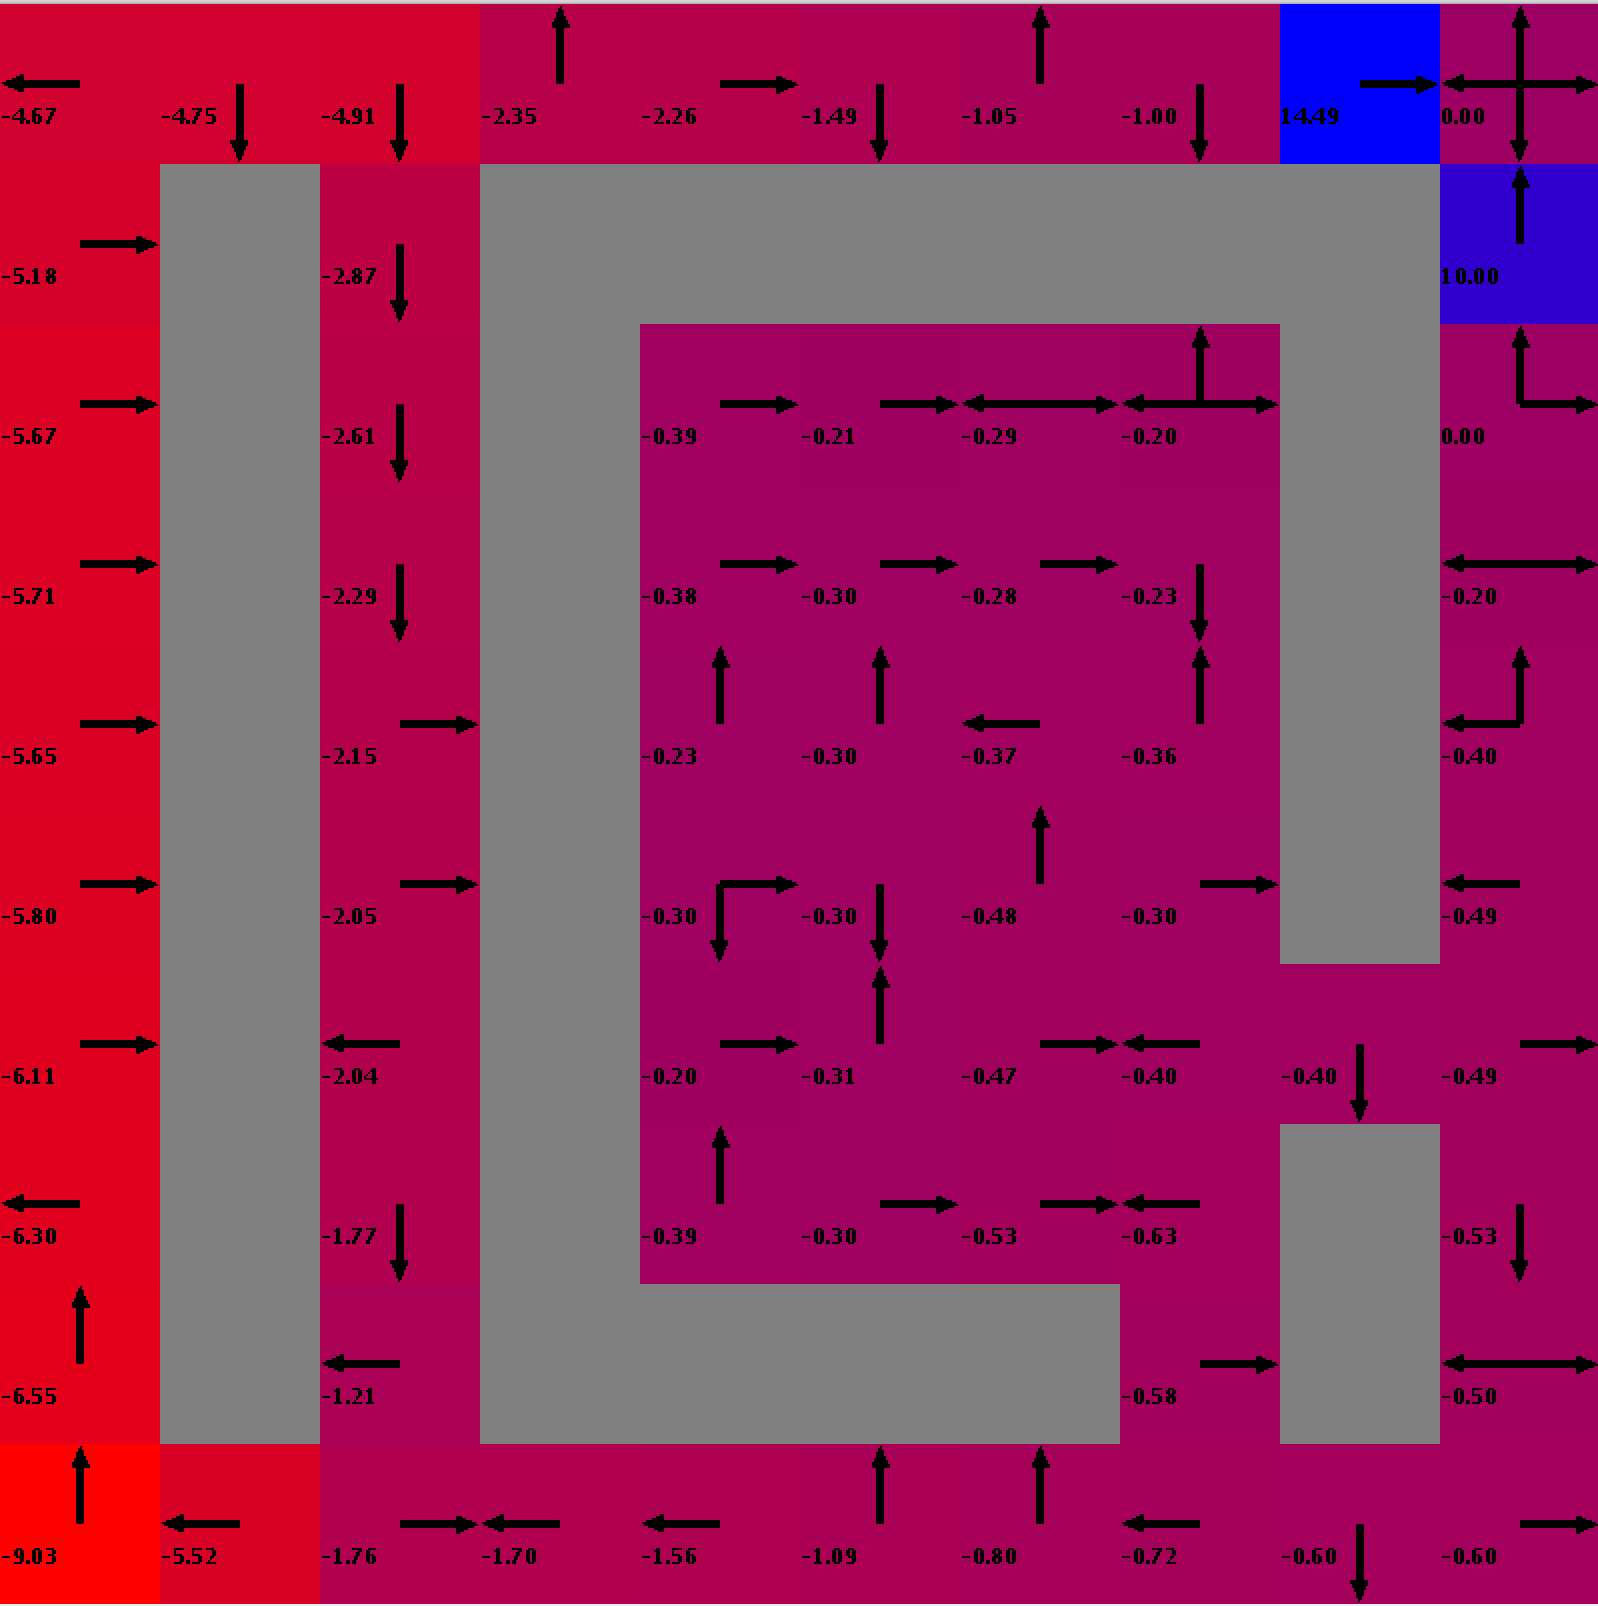
\includegraphics[width=1\textwidth,keepaspectratio]{easy-q-8.png} 
      \caption*{Easy GW Q-learning Iteration \#8} 
   \endminipage\hfill
   \minipage{0.245\textwidth}
      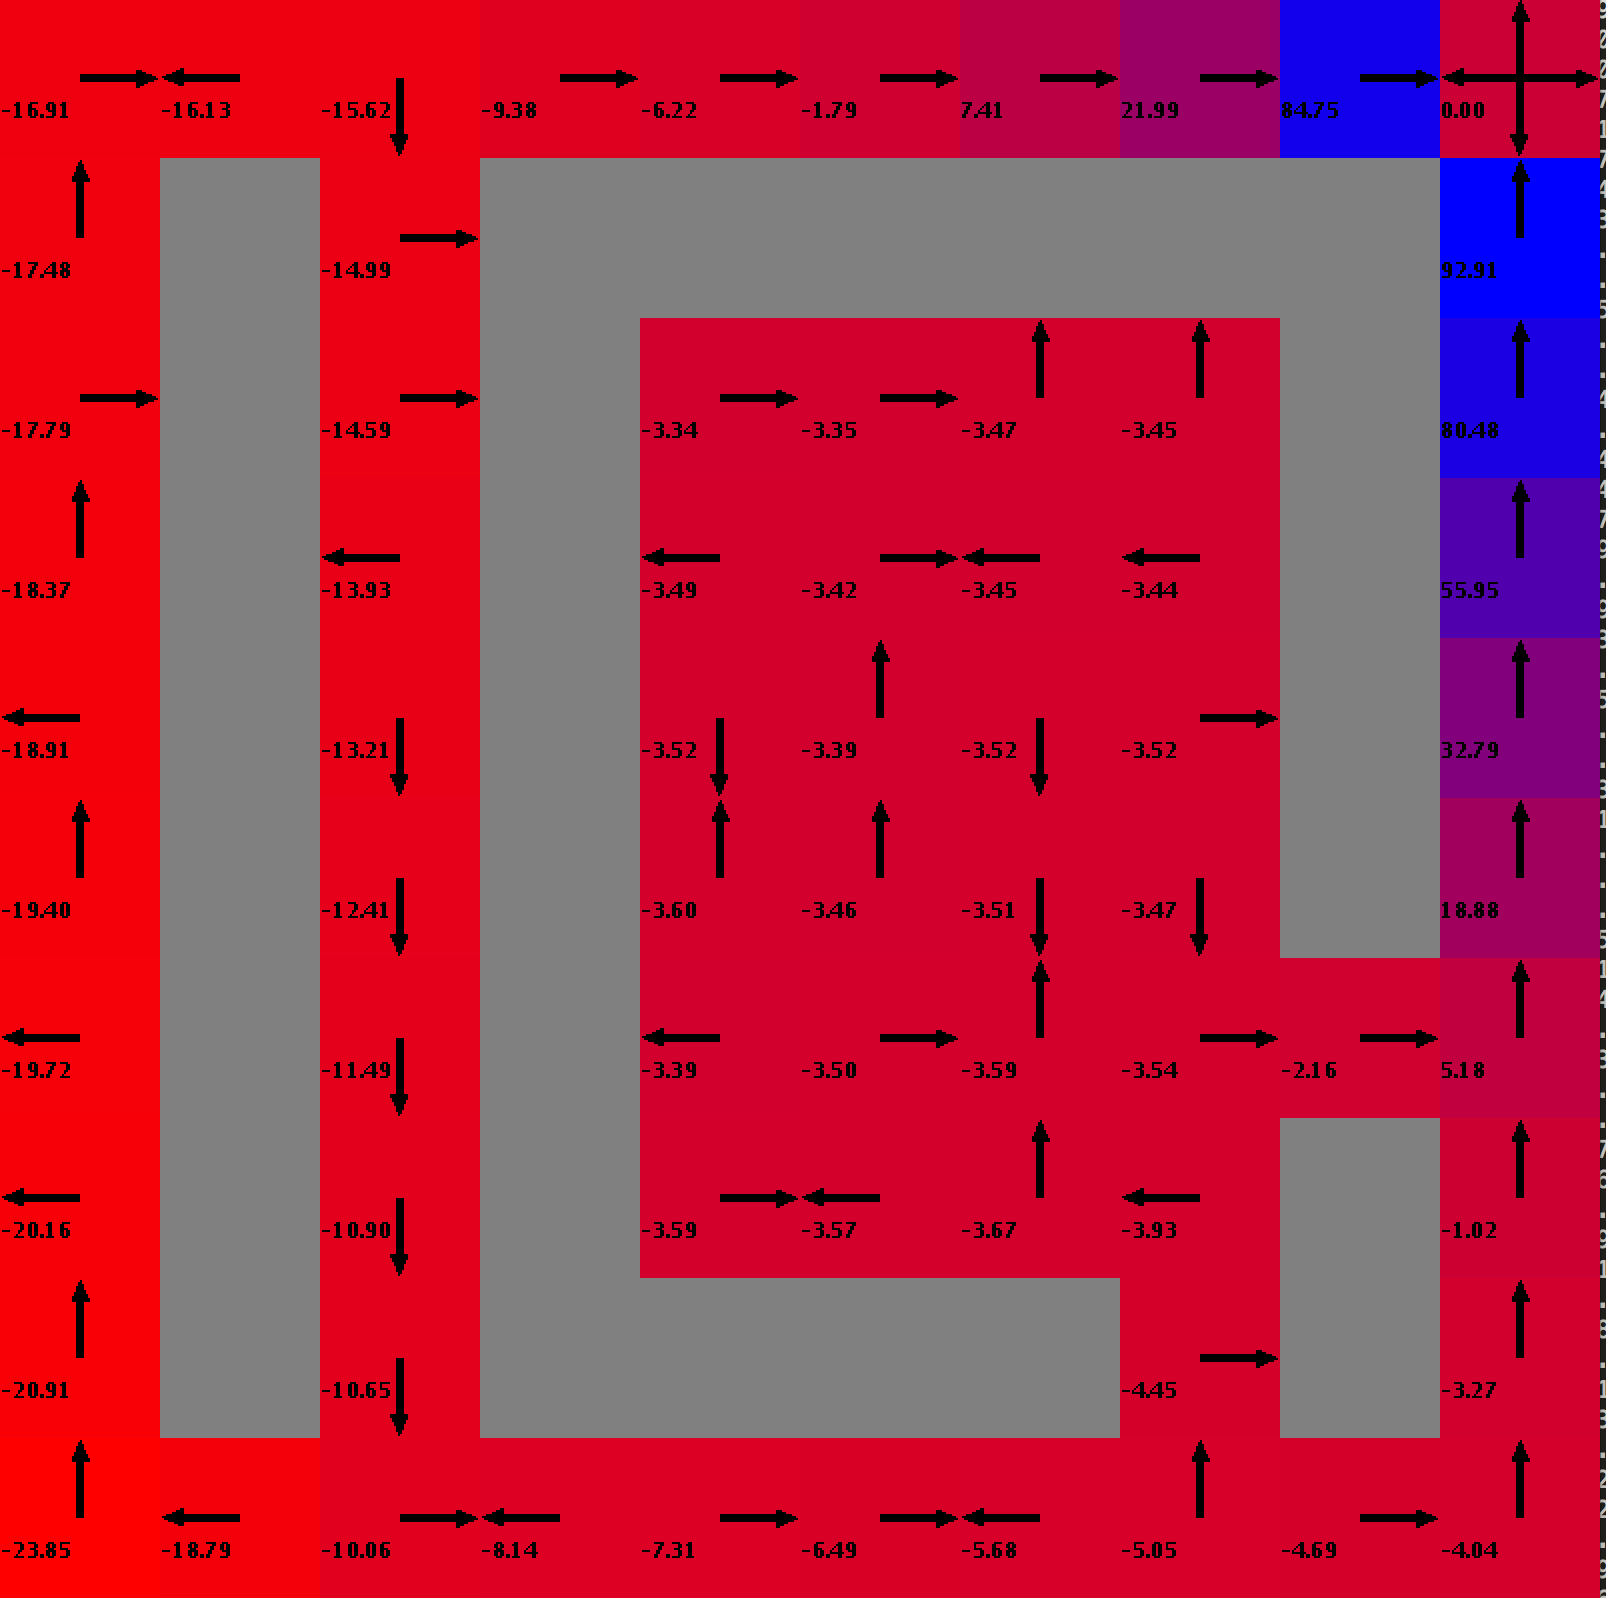
\includegraphics[width=1\textwidth,keepaspectratio]{easy-q-50.png} 
      \caption*{Easy GW Q-learning Iteration \#50} 
   \endminipage\hfill
   \minipage{0.245\textwidth}
      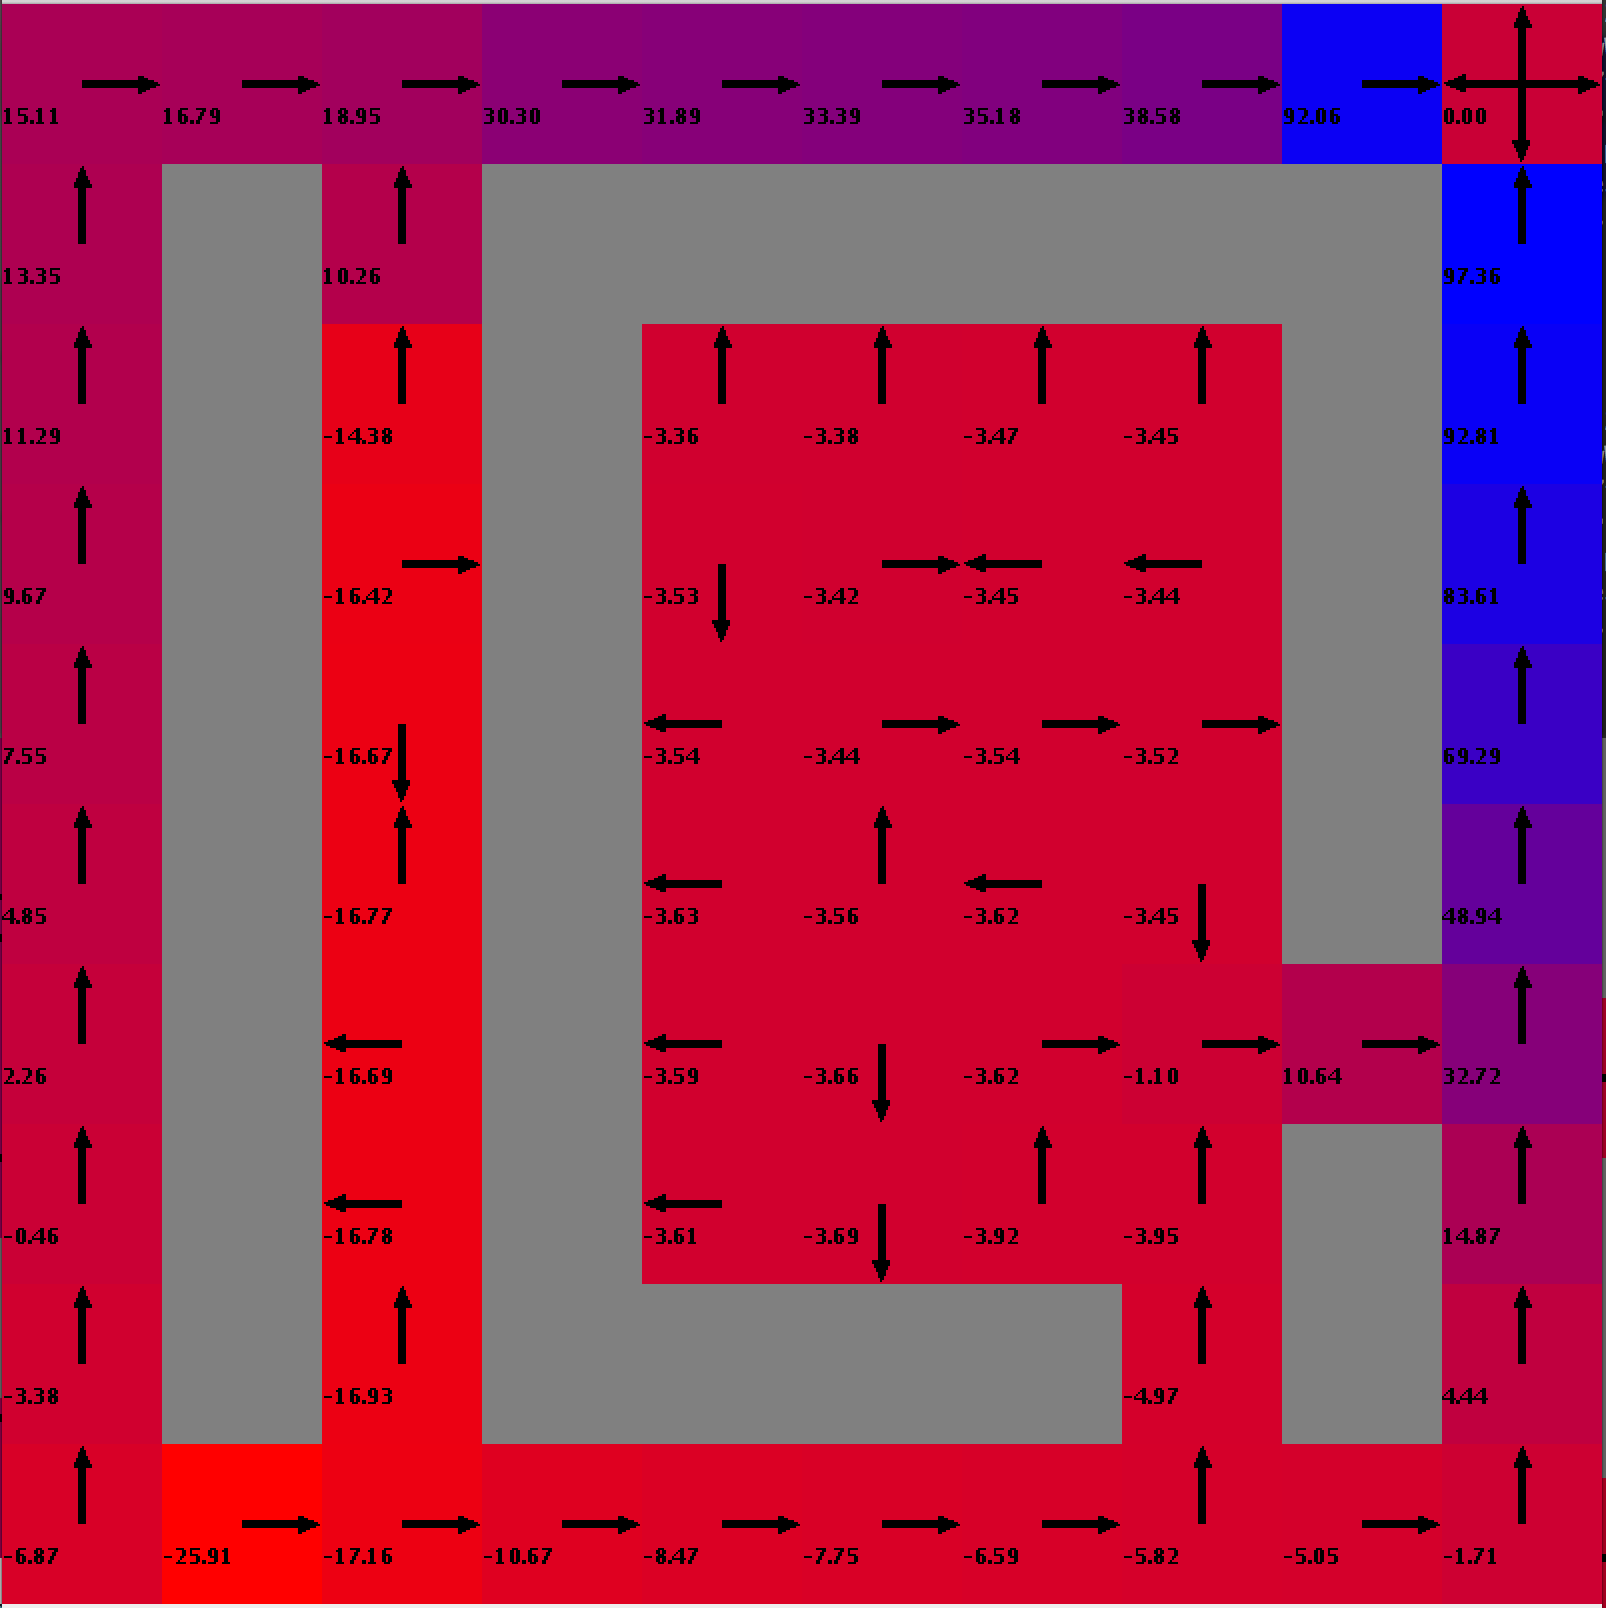
\includegraphics[width=1\textwidth,keepaspectratio]{easy-q-158.png} 
      \caption*{Easy GW Q-learning Iteration \#158} 
   \endminipage\hfill
   \minipage{0.245\textwidth}
      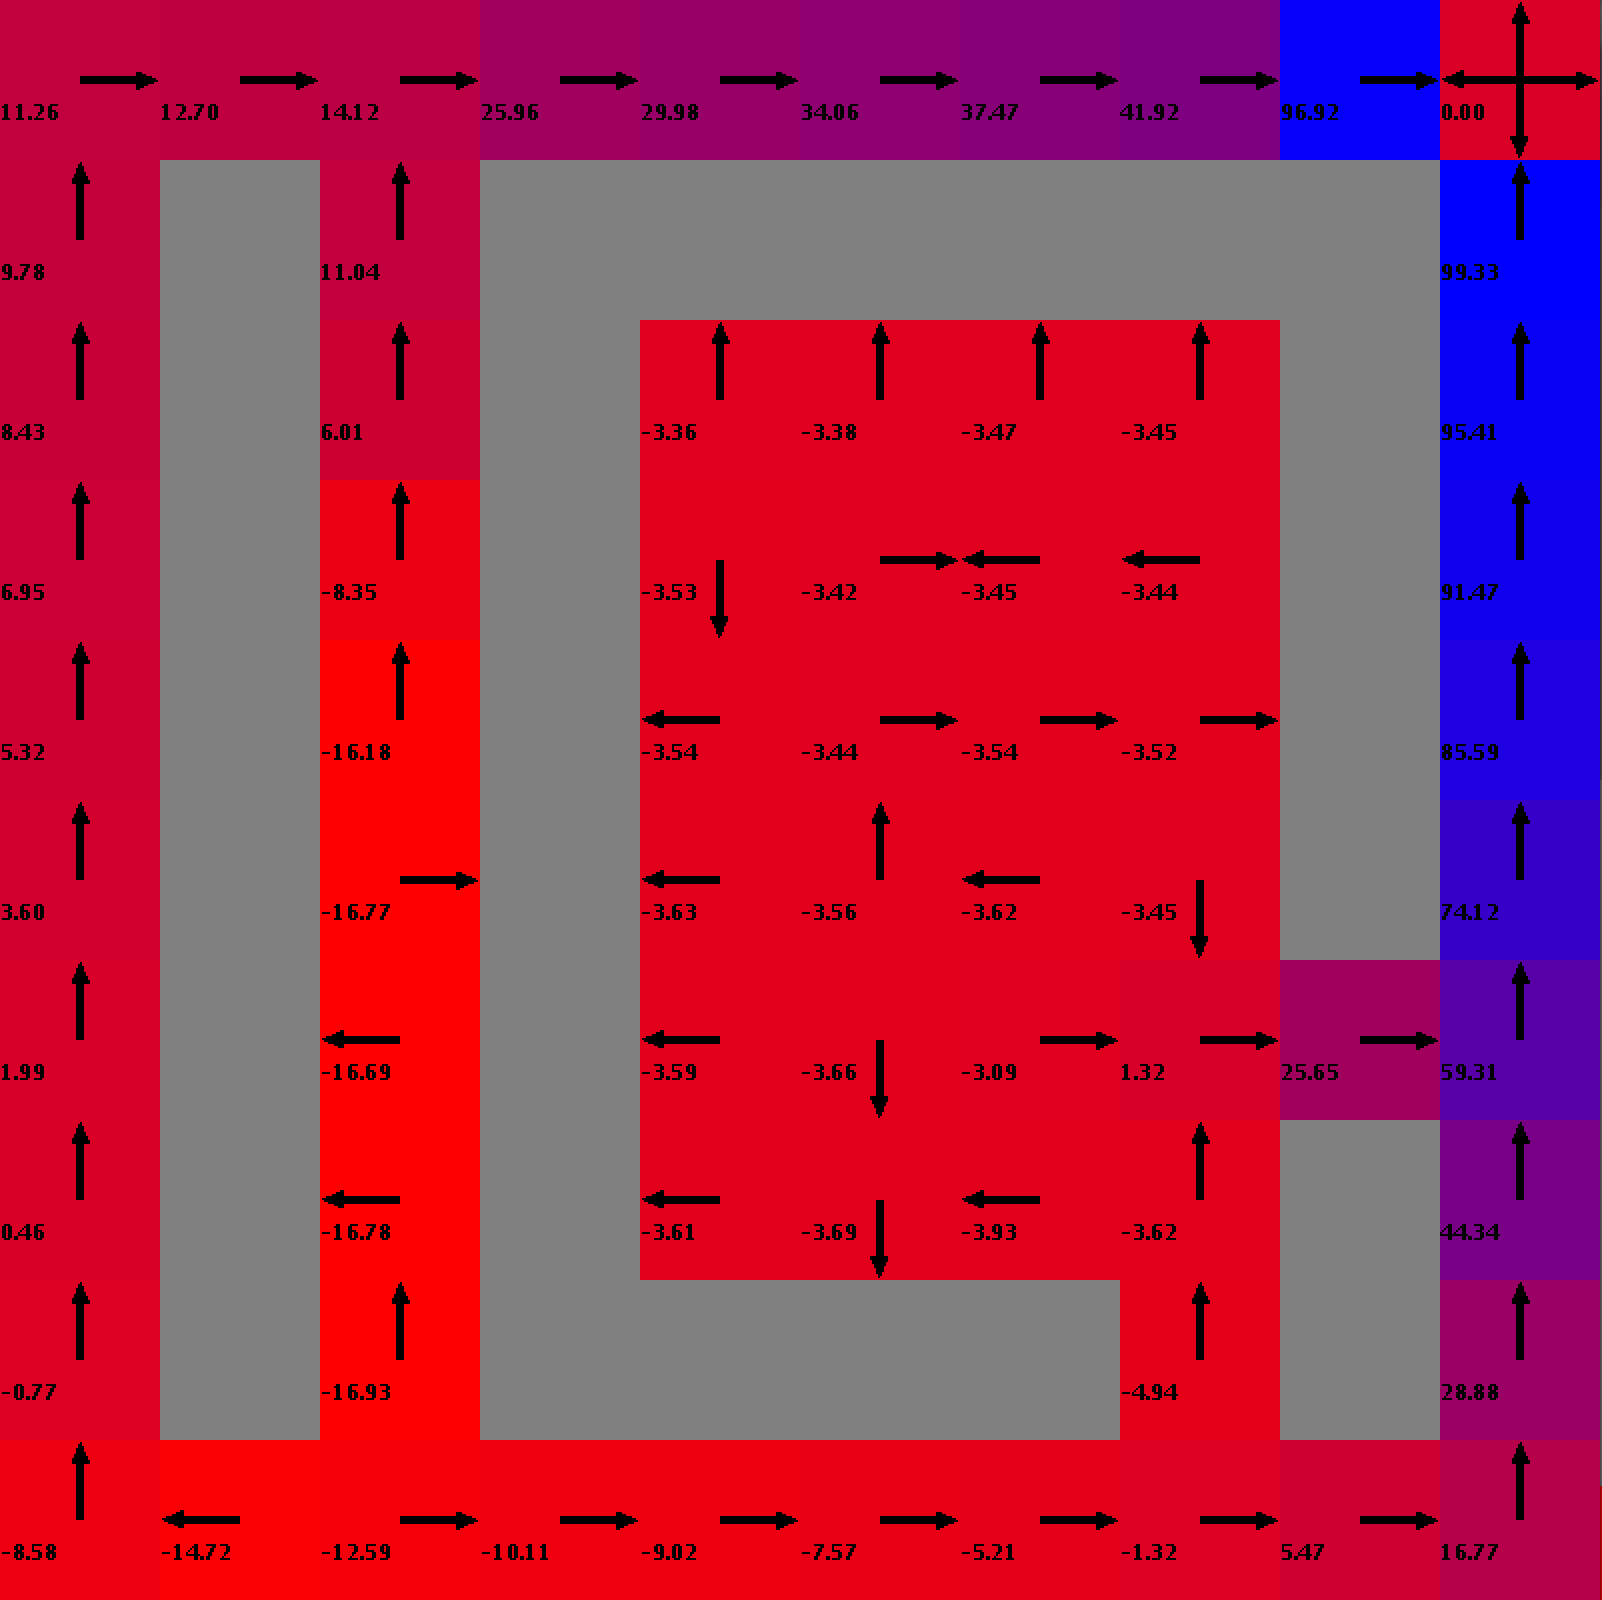
\includegraphics[width=1\textwidth,keepaspectratio]{easy-q-1000.png} 
      \caption*{Easy GW Q-learning Iteration \#1000} 
   \endminipage\hfill
\end{figure}


   \begin{figure}[H]
  \minipage{0.245\textwidth}
      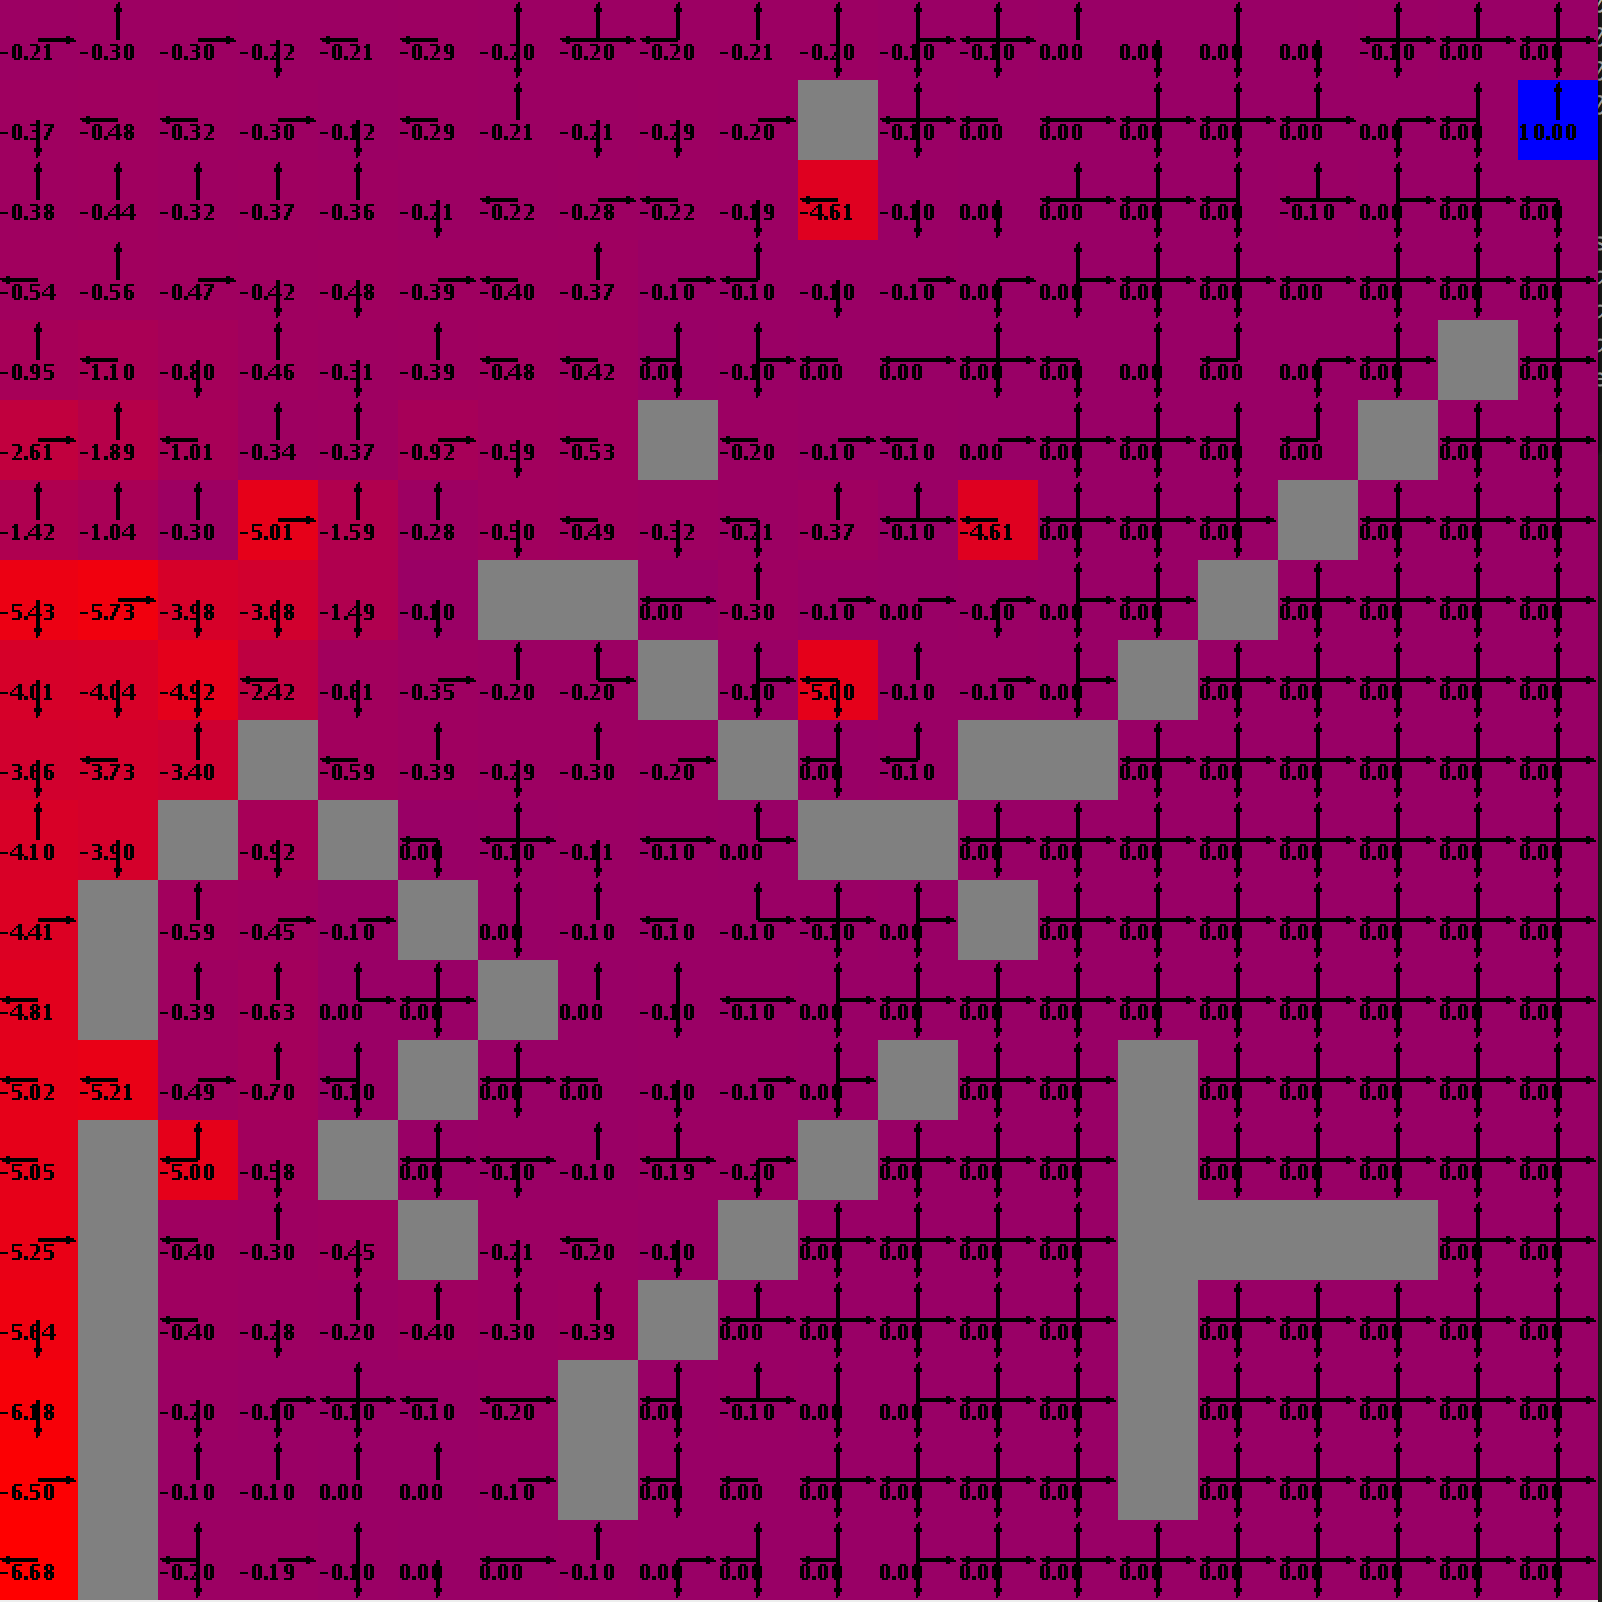
\includegraphics[width=1\textwidth,keepaspectratio]{hard-q-9.png} 
      \caption*{Hard GW Q-learning Iteration \#9} 
   \endminipage\hfill
   \minipage{0.245\textwidth}
      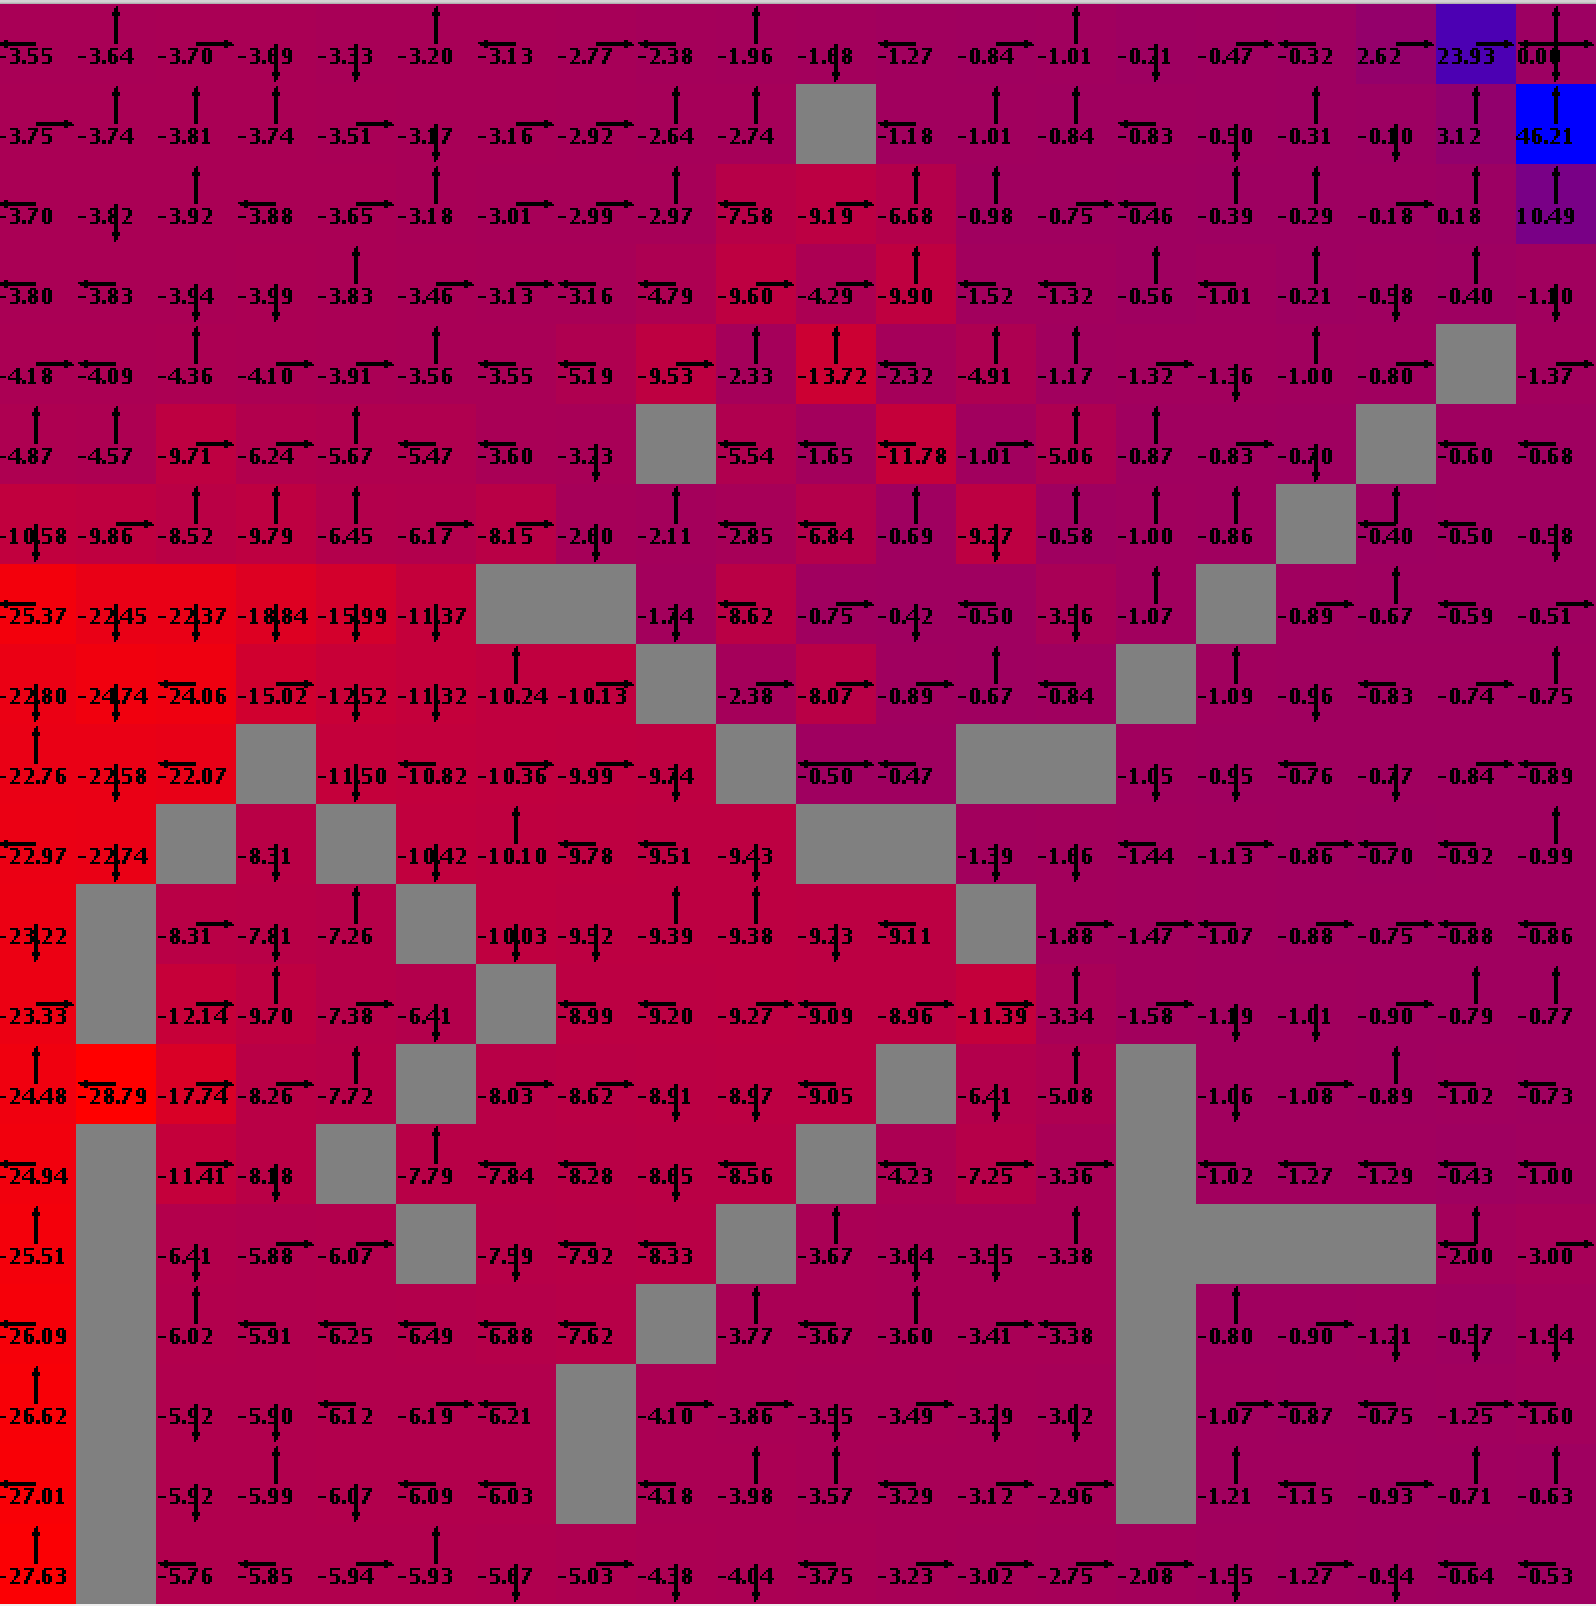
\includegraphics[width=1\textwidth,keepaspectratio]{hard-q-100.png} 
      \caption*{Hard GW Q-learning Iteration \#100} 
   \endminipage\hfill
   \minipage{0.245\textwidth}
      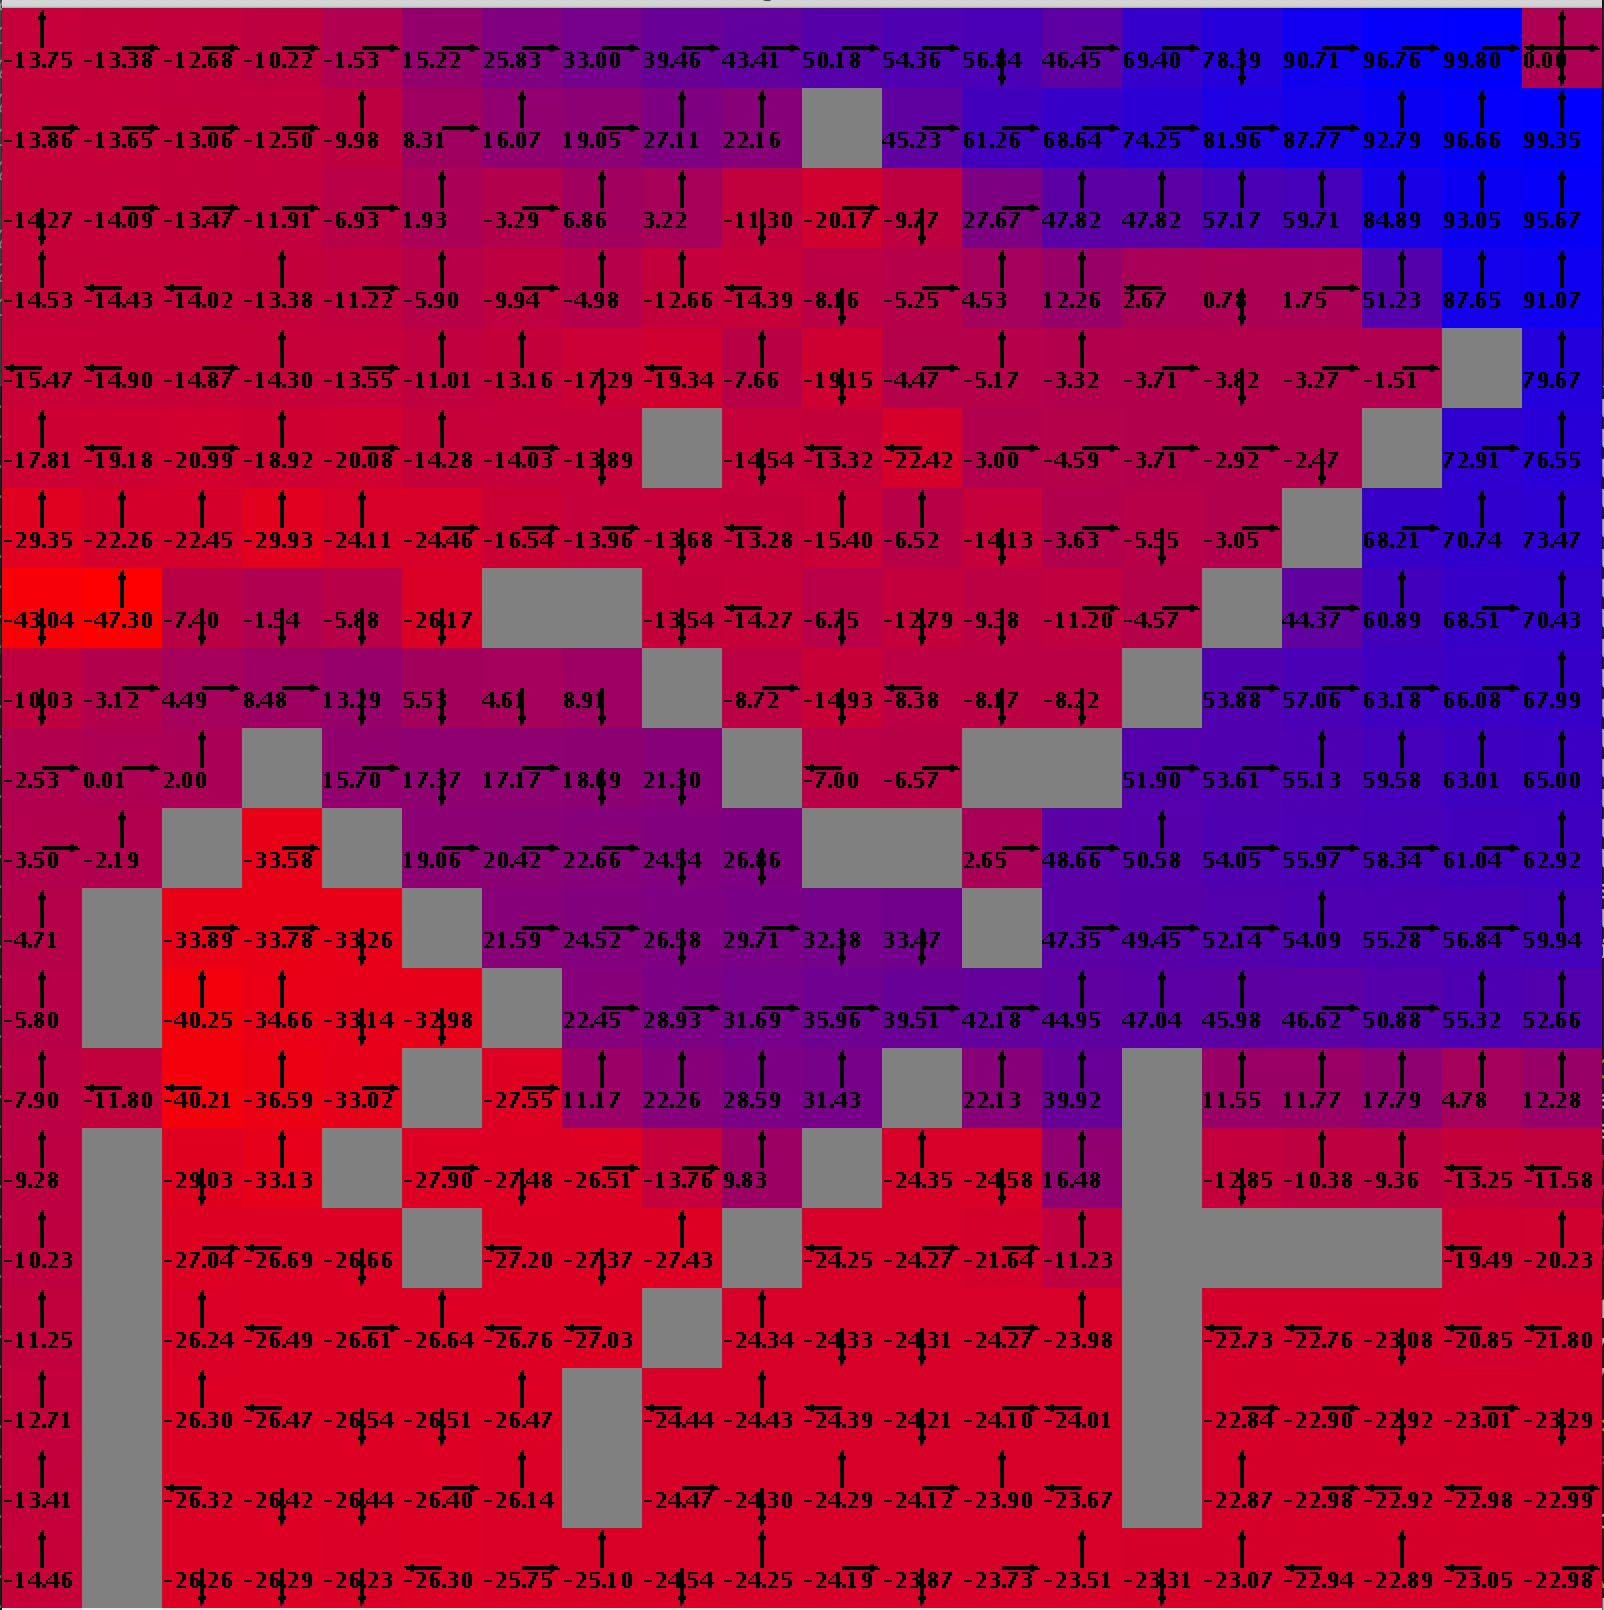
\includegraphics[width=1\textwidth,keepaspectratio]{hard-q-1066.png} 
      \caption*{Hard GW Q-learning Iteration \#1066} 
   \endminipage\hfill
   \minipage{0.245\textwidth}
      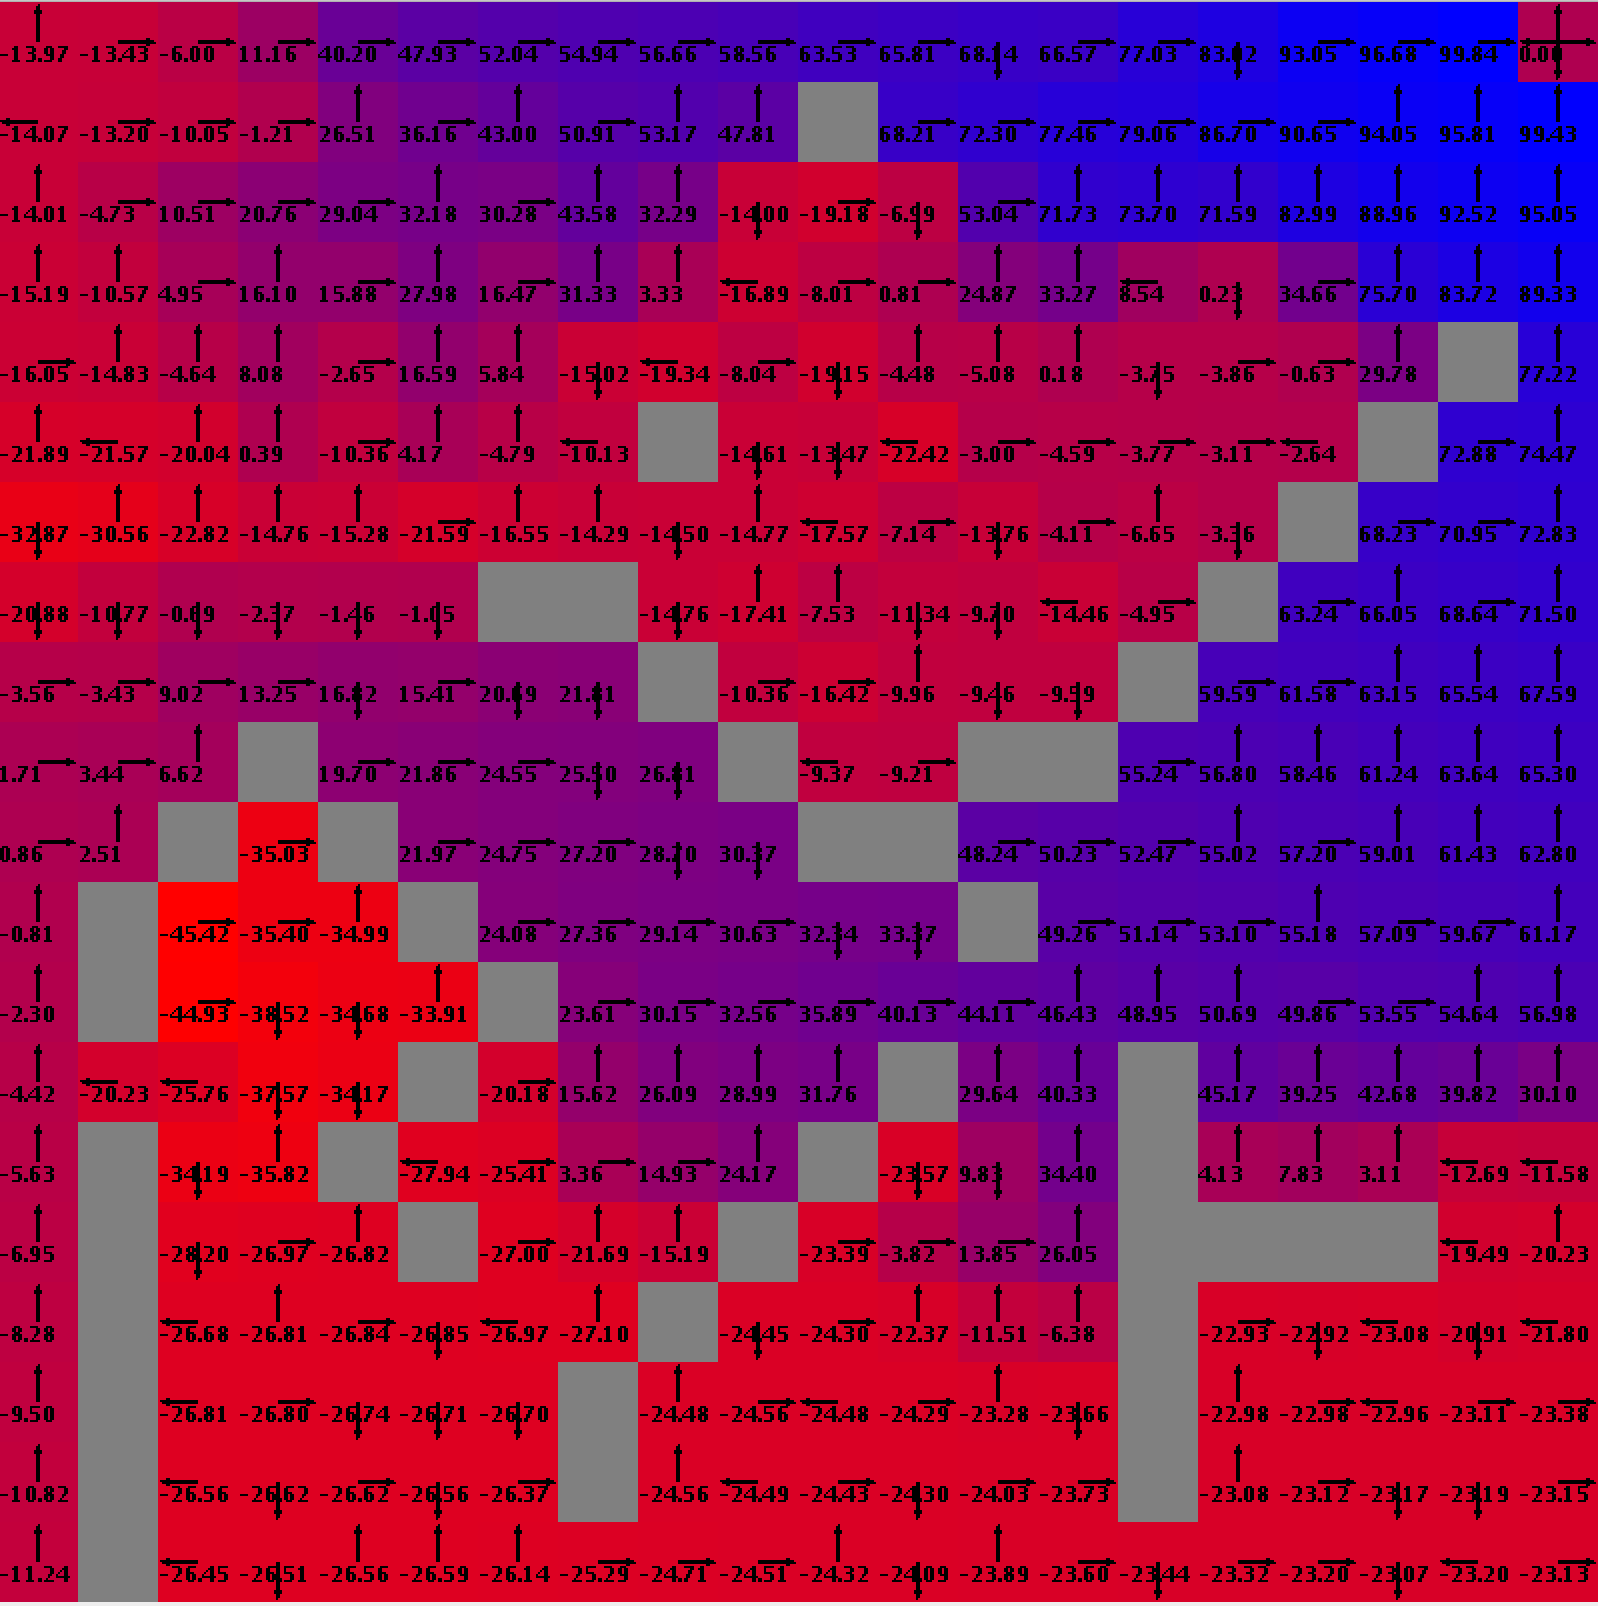
\includegraphics[width=1\textwidth,keepaspectratio]{hard-q-2900.png} 
      \caption*{Hard GW Q-learning Iteration \#2900} 
   \endminipage\hfill
\end{figure}


\section*{Comparison}

  \begin{figure}[H]
  \minipage{0.01\textwidth}
   \endminipage\hfill
  \minipage{0.49\textwidth}
      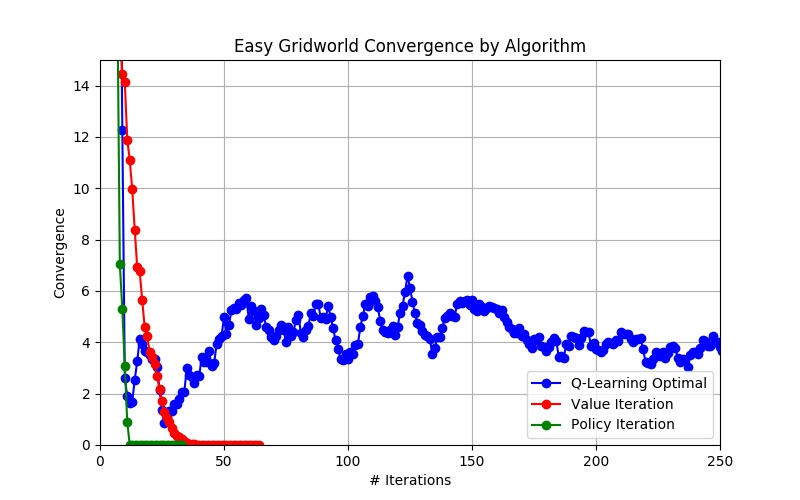
\includegraphics[width=1\textwidth,keepaspectratio]{easy_convergence.jpg} 
      \caption*{10x10 Easy Gridworld Convergence Comparison} 
   \endminipage\hfill
   \minipage{0.49\textwidth}
      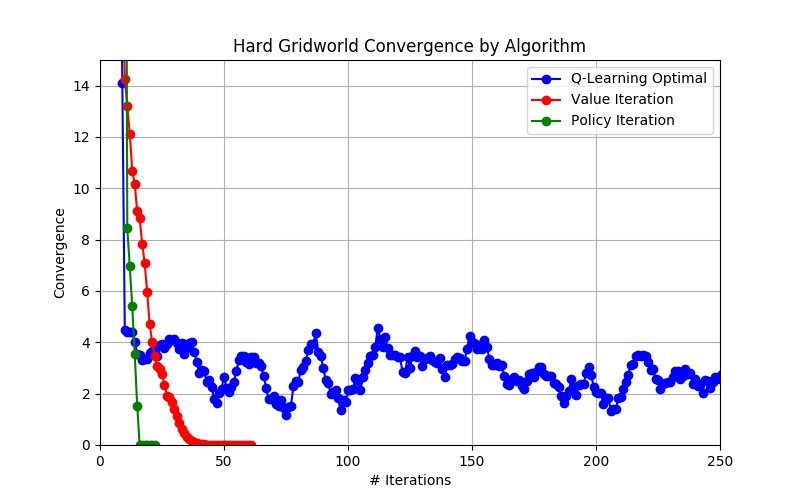
\includegraphics[width=1\textwidth,keepaspectratio]{hard_convergence.jpg} 
      \caption*{20x20 Hard Gridworld Convergence Comparison} 
   \endminipage\hfill
   \minipage{0.01\textwidth}
   \endminipage\hfill
\end{figure}

  \begin{figure}[H]
  \minipage{0.01\textwidth}
   \endminipage\hfill
  \minipage{0.49\textwidth}
      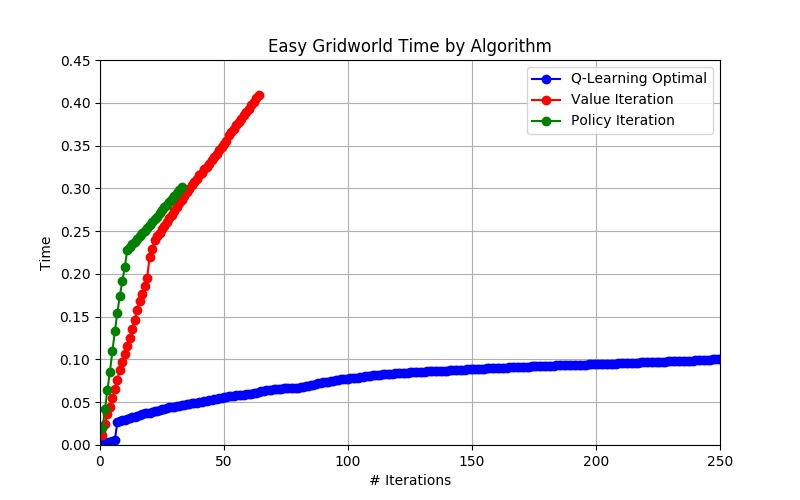
\includegraphics[width=1\textwidth,keepaspectratio]{easy_time.jpg} 
      \caption*{10x10 Easy Gridworld Time Comparison} 
   \endminipage\hfill
   \minipage{0.49\textwidth}
      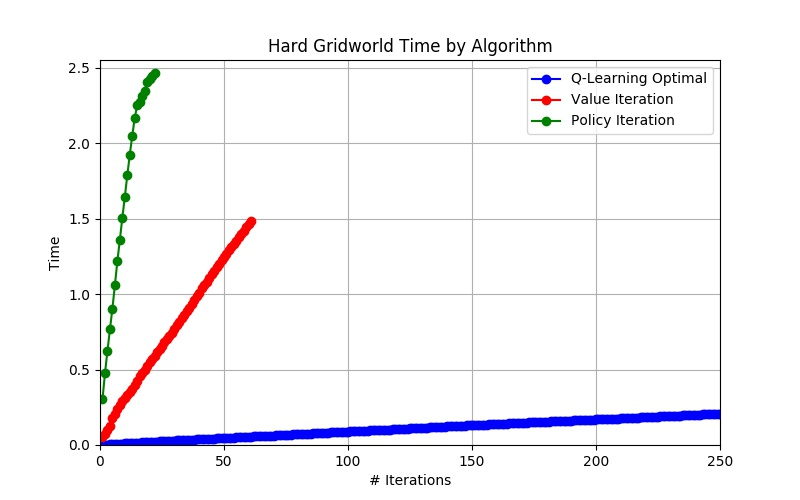
\includegraphics[width=1\textwidth,keepaspectratio]{hard_time.jpg} 
      \caption*{20x20 Hard Gridworld Time Comparison} 
   \endminipage\hfill
   \minipage{0.01\textwidth}
   \endminipage\hfill
\end{figure}


  \begin{figure}[H]
  \minipage{0.01\textwidth}
   \endminipage\hfill
  \minipage{0.49\textwidth}
      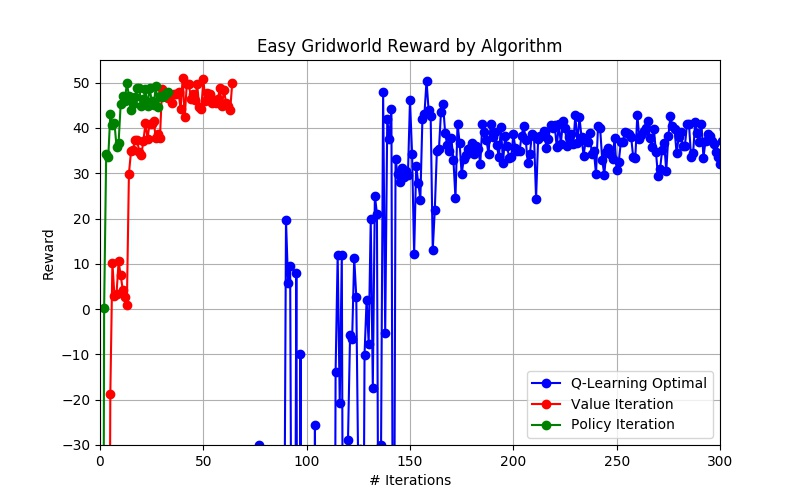
\includegraphics[width=1\textwidth,keepaspectratio]{easy_reward.jpg} 
      \caption*{10x10 Easy Gridworld Reward Comparison} 
   \endminipage\hfill
   \minipage{0.49\textwidth}
      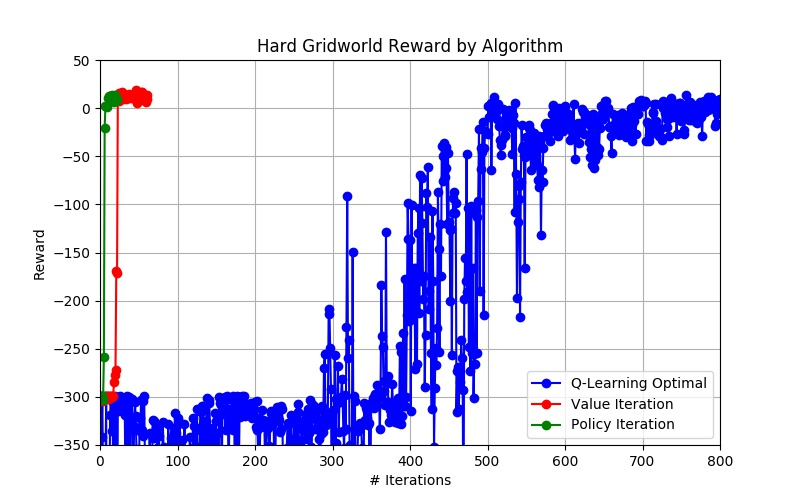
\includegraphics[width=1\textwidth,keepaspectratio]{hard_reward.jpg} 
      \caption*{20x20 Hard Gridworld Reward Comparison} 
   \endminipage\hfill
   \minipage{0.01\textwidth}
   \endminipage\hfill
\end{figure}



\end{document}